\documentclass[letter-paper]{tufte-book}

%%
% Book metadata
\title{Riemannian geometry 4H}
\author[]{B. S. H. Mithrandir}
%\publisher{Research Institute of Valinor}

%%
% If they're installed, use Bergamo and Chantilly from www.fontsite.com.
% They're clones of Bembo and Gill Sans, respectively.
\IfFileExists{bergamo.sty}{\usepackage[osf]{bergamo}}{}% Bembo
\IfFileExists{chantill.sty}{\usepackage{chantill}}{}% Gill Sans

%\usepackage{microtype}
\usepackage{amssymb}
\usepackage{amsmath}
%%
% For nicely typeset tabular material
\usepackage{booktabs}

%% overunder braces
\usepackage{oubraces}

%% 
\usepackage{xcolor}
\usepackage{tcolorbox}

\newtcolorbox[auto counter,number within=section]{derivbox}[2][]{colback=TealBlue!5!white,colframe=TealBlue,title=Box \thetcbcounter:\ #2,#1}                                                          

\makeatletter
\@openrightfalse
\makeatother

%%
% For graphics / images
\usepackage{graphicx}
\setkeys{Gin}{width=\linewidth,totalheight=\textheight,keepaspectratio}
\graphicspath{{figs/}}

\usepackage{tikz-cd}

% The fancyvrb package lets us customize the formatting of verbatim
% environments.  We use a slightly smaller font.
\usepackage{fancyvrb}
\fvset{fontsize=\normalsize}

\usepackage[plain]{fancyref}
\newcommand*{\fancyrefboxlabelprefix}{box}
\fancyrefaddcaptions{english}{%
  \providecommand*{\frefboxname}{Box}%
  \providecommand*{\Frefboxname}{Box}%
}
\frefformat{plain}{\fancyrefboxlabelprefix}{\frefboxname\fancyrefdefaultspacing#1}
\Frefformat{plain}{\fancyrefboxlabelprefix}{\Frefboxname\fancyrefdefaultspacing#1}

%%
% Prints argument within hanging parentheses (i.e., parentheses that take
% up no horizontal space).  Useful in tabular environments.
\newcommand{\hangp}[1]{\makebox[0pt][r]{(}#1\makebox[0pt][l]{)}}

%% 
% Prints an asterisk that takes up no horizontal space.
% Useful in tabular environments.
\newcommand{\hangstar}{\makebox[0pt][l]{*}}

%%
% Prints a trailing space in a smart way.
\usepackage{xspace}
\usepackage{xstring}

%%
% Some shortcuts for Tufte's book titles.  The lowercase commands will
% produce the initials of the book title in italics.  The all-caps commands
% will print out the full title of the book in italics.
\newcommand{\vdqi}{\textit{VDQI}\xspace}
\newcommand{\ei}{\textit{EI}\xspace}
\newcommand{\ve}{\textit{VE}\xspace}
\newcommand{\be}{\textit{BE}\xspace}
\newcommand{\VDQI}{\textit{The Visual Display of Quantitative Information}\xspace}
\newcommand{\EI}{\textit{Envisioning Information}\xspace}
\newcommand{\VE}{\textit{Visual Explanations}\xspace}
\newcommand{\BE}{\textit{Beautiful Evidence}\xspace}

\newcommand{\TL}{Tufte-\LaTeX\xspace}

% Prints the month name (e.g., January) and the year (e.g., 2008)
\newcommand{\monthyear}{%
  \ifcase\month\or January\or February\or March\or April\or May\or June\or
  July\or August\or September\or October\or November\or
  December\fi\space\number\year
}


\newcommand{\urlwhitespacereplace}[1]{\StrSubstitute{#1}{ }{_}[\wpLink]}

\newcommand{\wikipedialink}[1]{http://en.wikipedia.org/wiki/#1}% needs \wpLink now

\newcommand{\anonymouswikipedialink}[1]{\urlwhitespacereplace{#1}\href{\wikipedialink{\wpLink}}{Wikipedia}}

\newcommand{\Wikiref}[1]{\urlwhitespacereplace{#1}\href{\wikipedialink{\wpLink}}{#1}}

% Prints an epigraph and speaker in sans serif, all-caps type.
\newcommand{\openepigraph}[2]{%
  %\sffamily\fontsize{14}{16}\selectfont
  \begin{fullwidth}
  \sffamily\large
  \begin{doublespace}
  \noindent\allcaps{#1}\\% epigraph
  \noindent\allcaps{#2}% author
  \end{doublespace}
  \end{fullwidth}
}

% Inserts a blank page
\newcommand{\blankpage}{\newpage\hbox{}\thispagestyle{empty}\newpage}

\usepackage{units}

% Typesets the font size, leading, and measure in the form of 10/12x26 pc.
\newcommand{\measure}[3]{#1/#2$\times$\unit[#3]{pc}}

% Macros for typesetting the documentation
\newcommand{\hlred}[1]{\textcolor{Maroon}{#1}}% prints in red
\newcommand{\hangleft}[1]{\makebox[0pt][r]{#1}}
\newcommand{\hairsp}{\hspace{1pt}}% hair space
\newcommand{\hquad}{\hskip0.5em\relax}% half quad space
\newcommand{\TODO}{\textcolor{red}{\bf TODO!}\xspace}
\newcommand{\na}{\quad--}% used in tables for N/A cells
\providecommand{\XeLaTeX}{X\lower.5ex\hbox{\kern-0.15em\reflectbox{E}}\kern-0.1em\LaTeX}
\newcommand{\tXeLaTeX}{\XeLaTeX\index{XeLaTeX@\protect\XeLaTeX}}
% \index{\texttt{\textbackslash xyz}@\hangleft{\texttt{\textbackslash}}\texttt{xyz}}
\newcommand{\tuftebs}{\symbol{'134}}% a backslash in tt type in OT1/T1
\newcommand{\doccmdnoindex}[2][]{\texttt{\tuftebs#2}}% command name -- adds backslash automatically (and doesn't add cmd to the index)
\newcommand{\doccmddef}[2][]{%
  \hlred{\texttt{\tuftebs#2}}\label{cmd:#2}%
  \ifthenelse{\isempty{#1}}%
    {% add the command to the index
      \index{#2 command@\protect\hangleft{\texttt{\tuftebs}}\texttt{#2}}% command name
    }%
    {% add the command and package to the index
      \index{#2 command@\protect\hangleft{\texttt{\tuftebs}}\texttt{#2} (\texttt{#1} package)}% command name
      \index{#1 package@\texttt{#1} package}\index{packages!#1@\texttt{#1}}% package name
    }%
}% command name -- adds backslash automatically
\newcommand{\doccmd}[2][]{%
  \texttt{\tuftebs#2}%
  \ifthenelse{\isempty{#1}}%
    {% add the command to the index
      \index{#2 command@\protect\hangleft{\texttt{\tuftebs}}\texttt{#2}}% command name
    }%
    {% add the command and package to the index
      \index{#2 command@\protect\hangleft{\texttt{\tuftebs}}\texttt{#2} (\texttt{#1} package)}% command name
      \index{#1 package@\texttt{#1} package}\index{packages!#1@\texttt{#1}}% package name
    }%
}% command name -- adds backslash automatically
\newcommand{\docopt}[1]{\ensuremath{\langle}\textrm{\textit{#1}}\ensuremath{\rangle}}% optional command argument
\newcommand{\docarg}[1]{\textrm{\textit{#1}}}% (required) command argument
\newenvironment{docspec}{\begin{quotation}\ttfamily\parskip0pt\parindent0pt\ignorespaces}{\end{quotation}}% command specification environment
\newcommand{\docenv}[1]{\texttt{#1}\index{#1 environment@\texttt{#1} environment}\index{environments!#1@\texttt{#1}}}% environment name
\newcommand{\docenvdef}[1]{\hlred{\texttt{#1}}\label{env:#1}\index{#1 environment@\texttt{#1} environment}\index{environments!#1@\texttt{#1}}}% environment name
\newcommand{\docpkg}[1]{\texttt{#1}\index{#1 package@\texttt{#1} package}\index{packages!#1@\texttt{#1}}}% package name
\newcommand{\doccls}[1]{\texttt{#1}}% document class name
\newcommand{\docclsopt}[1]{\texttt{#1}\index{#1 class option@\texttt{#1} class option}\index{class options!#1@\texttt{#1}}}% document class option name
\newcommand{\docclsoptdef}[1]{\hlred{\texttt{#1}}\label{clsopt:#1}\index{#1 class option@\texttt{#1} class option}\index{class options!#1@\texttt{#1}}}% document class option name defined
\newcommand{\docmsg}[2]{\bigskip\begin{fullwidth}\noindent\ttfamily#1\end{fullwidth}\medskip\par\noindent#2}
\newcommand{\docfilehook}[2]{\texttt{#1}\index{file hooks!#2}\index{#1@\texttt{#1}}}
\newcommand{\doccounter}[1]{\texttt{#1}\index{#1 counter@\texttt{#1} counter}}

\newcommand{\studyq}[1]{\marginnote{Q: #1}}

\hypersetup{colorlinks}% uncomment this line if you prefer colored hyperlinks (e.g., for onscreen viewing)

% Generates the index
\usepackage{makeidx}
\makeindex

\setcounter{tocdepth}{3}
\setcounter{secnumdepth}{3}

%%%%%%%%%%%%%%%%%%%%%%%%%%%%%%%%%%%%%%%%%%%%%%%%%%%%%%%%%%%%%%
% custom commands

\newtheorem{theorem}{\color{pastel-blue}Theorem}[section]
\newtheorem{lemma}[theorem]{\color{pastel-blue}Lemma}
\newtheorem{proposition}[theorem]{\color{pastel-blue}Proposition}
\newtheorem{corollary}[theorem]{\color{pastel-blue}Corollary}

\newenvironment{proof}[1][Proof]{\begin{trivlist}
\item[\hskip \labelsep {\bfseries #1}]}{\end{trivlist}}
\newenvironment{definition}[1][Definition]{\begin{trivlist}
\item[\hskip \labelsep {\bfseries #1}]}{\end{trivlist}}
\newenvironment{example}[1][Example]{\begin{trivlist}
\item[\hskip \labelsep {\bfseries #1}]}{\end{trivlist}}
\newenvironment{remark}[1][Remark]{\begin{trivlist}
\item[\hskip \labelsep {\bfseries #1}]}{\end{trivlist}}

\hyphenpenalty=5000

% more pastel ones
\xdefinecolor{pastel-red}{rgb}{0.77,0.31,0.32}
\xdefinecolor{pastel-green}{rgb}{0.33,0.66,0.41}
\definecolor{pastel-blue}{rgb}{0.30,0.45,0.69} % crayola blue
\definecolor{gray}{rgb}{0.2,0.2,0.2} % dark gray

\xdefinecolor{orange}{rgb}{1,0.45,0}
\xdefinecolor{green}{rgb}{0,0.35,0}
\definecolor{blue}{rgb}{0.12,0.46,0.99} % crayola blue
\definecolor{gray}{rgb}{0.2,0.2,0.2} % dark gray

\xdefinecolor{cerulean}{rgb}{0.01,0.48,0.65}
\xdefinecolor{ust-blue}{rgb}{0,0.20,0.47}
\xdefinecolor{ust-mustard}{rgb}{0.67,0.52,0.13}

%\newcommand\comment[1]{{\color{red}#1}}

\newcommand{\dy}{\partial}
\newcommand{\ddy}[2]{\frac{\dy#1}{\dy#2}}

\newcommand{\ex}{\mathrm{e}}
\newcommand{\zi}{{\rm i}}

\newcommand\Real{\mbox{Re}} % cf plain TeX's \Re and Reynolds number
\newcommand\Imag{\mbox{Im}} % cf plain TeX's \Im

\newcommand\Def[1]{\textbf{#1}}

\newcommand{\qed}{\hfill$\blacksquare$}
\newcommand{\qedwhite}{\hfill \ensuremath{\Box}}

\newcommand{\highlight}[1]{\mathchoice%
  {\colorbox{black!10}{$\displaystyle#1$}}%
  {\colorbox{black!10}{$\textstyle#1$}}%
  {\colorbox{black!10}{$\scriptstyle#1$}}%
  {\colorbox{black!10}{$\scriptscriptstyle#1$}}}%

%%%%%%%%%%%%%%%%%%%%%%%%%%%%%%%%%%%%%%%%%%%%%%%%%%%%%%%%%%%%%%
% some extra formatting (hacked from Patrick Farrell's notes)
%  https://courses.maths.ox.ac.uk/node/view_material/4915
%

% chapter format
\titleformat{\chapter}%
  {\huge\rmfamily\itshape\color{pastel-red}}% format applied to label+text
  {\llap{\colorbox{pastel-red}{\parbox{1.5cm}{\hfill\itshape\huge\color{white}\thechapter}}}}% label
  {1em}% horizontal separation between label and title body
  {}% before the title body
  []% after the title body

% section format
\titleformat{\section}%
  {\normalfont\Large\itshape\color{pastel-green}}% format applied to label+text
  {\llap{\colorbox{pastel-green}{\parbox{1.5cm}{\hfill\color{white}\thesection}}}}% label
  {1em}% horizontal separation between label and title body
  {}% before the title body
  []% after the title body

% subsection format
\titleformat{\subsection}%
  {\normalfont\large\itshape\color{pastel-blue}}% format applied to label+text
  {\llap{\colorbox{pastel-blue}{\parbox{1.5cm}{\hfill\color{white}\thesubsection}}}}% label
  {1em}% horizontal separation between label and title body
  {}% before the title body
  []% after the title body

%%%%%%%%%%%%%%%%%%%%%%%%%%%%%%%%%%%%%%%%%%%%%%%%%%%%%%%%%%%%%%%%%%%%%%%%%%%%%%%%

\begin{document}

% Front matter
%\frontmatter

% r.3 full title page
%\maketitle

% v.4 copyright page

\chapter*{}

\begin{fullwidth}

\par \begin{center}{\Huge Riemannian geometry 4H}\end{center}

\vspace*{5mm}

\par \begin{center}{\Large typed up by B. S. H. Mithrandir}\end{center}

\vspace*{5mm}

\begin{itemize}
  \item \textit{Last compiled: \monthyear}
  \item Adapted from notes of (I think?) W. Klingenberg, Durham
  \item This was part of the Riemannian Geometric 4H module elective, as a follow on to the Differential geometry 3H course. Probably would help having gone through the Analysis 3H course also.
  \item[]
  \item \TODO diagrams
\end{itemize}

\par

\par Licensed under the Apache License, Version 2.0 (the ``License''); you may not
use this file except in compliance with the License. You may obtain a copy
of the License at \url{http://www.apache.org/licenses/LICENSE-2.0}. Unless
required by applicable law or agreed to in writing, software distributed
under the License is distributed on an \smallcaps{``AS IS'' BASIS, WITHOUT
WARRANTIES OR CONDITIONS OF ANY KIND}, either express or implied. See the
License for the specific language governing permissions and limitations
under the License.
\end{fullwidth}


%===============================================================================

\chapter{Differentiable manifolds}

Recall that a $k$-manifold $M$ is one which, locally, looked like open sets of $\mathbb{R}^k$. The manifold is build up by patching together these local sets.

\begin{example}
  \begin{enumerate}
    \item A surface of revoluation $M$ with $\gamma : [a, b] \to \mathbb {R}^3$ with $\gamma(t) = (\gamma_1(t), 0, \gamma_3(t))$ (assuming $\gamma'(t) \neq 0$ for all $t$ and $\gamma$ is simple) is given by
    \begin{align*}
      M &= \{ (\gamma_1(t), \gamma_3(t)\cos\theta, \gamma_3(t)\sin\theta)\ |\ t\in[a,b],\ \theta \in [0, 2\pi]\}\\
        &= \{ (x_1, x_2, x_3)\ |\ \exists t\in(a,b),\ x_1 = \gamma_1(t),\ x_2^2 + x_3^2 = \gamma_3^2(t)\}.
    \end{align*}
    
    \item The matrix group $\mbox{SL}(n, \mathbb{R})$, $\mbox{O}(n)$ and $\mbox{SO}(n)$ can be considered as submanifolds of the ambient space $\mathbb{R}^{n^2} = M(n, \mathbb{R}$.
    
    \item The real projective plane/space $\mathbb{R}\mbox{P}^n$ is given by the set of all lines through the origin in $\mathbb{R}^{n+1}$. It can be identified with the quotient group $S^n / \sim$, where $p \sim q$ iff $p = \pm q$.
  \end{enumerate}
\end{example}

Recall that for an $n$-dimensional subspace $X \subset \mathbb{R}^n$, $x \in X$ is called an \textbf{inner point} of iff there exists an $n$-dimensional open $U \subset X$ with $x\in U$. $X$ is \textbf{open} if every $x \in X$ is an inner point.

Let $M$ be a set. A collection $(U_\alpha, \phi_\alpha)$ with index $\alpha$ is called an \textbf{atlas} of $M$ is
\begin{enumerate}
  \item $U_\alpha \in M$ and $\bigcup_\alpha U_\alpha = M$ (the collection of $U_\alpha$ covers $M$),
  
  \item $\phi_\alpha : U_\alpha \to V_\alpha \subset \mathbb{R}^n$ are bijective maps with open $V_\alpha$, and for each $\alpha, \beta$, $\phi_\alpha(U_\alpha \cap U_\beta)$ is open,
  
  \item the co-ordinate changes $\phi_\beta \circ \phi_\alpha^{-1} : \phi_\alpha(U_\alpha \cap U_\beta) \to \phi_\beta(U_\alpha \cap U_\beta)$ are smooth maps between open subsets of $\mathbb{R}^n$.
\end{enumerate}

Let $(U_\alpha, \phi_\alpha)$ be an atlas of $M$, and $X \subset M$. A point $x \in X$ is called an \textbf{inner point} of $X$ is there exists $\phi_\alpha : U_\alpha \to V_\alpha \subset \mathbb{R}^n$ such that $\phi_\alpha(x)$ is an inner point of $\phi_\alpha (X \cap U_\alpha)$ for $x \in U_\alpha$. $X$ is \textbf{open} if every $x \in X$ is an inner point.

A set $M$ is a \textbf{differentiable manifold} if it carries an atlas $(U_\alpha, \phi_\alpha)$ and has the \textbf{Hausdorff property}, i.e. for any $p, q \in M$ with $p \neq q$, there exists open $A_p, A_q \subset M$ such that for $p \in A_p$ and $q \in A_q$ where $A_p \cap A_q = \emptyset$.\marginnote{This would be the $T_2$ condition relating to topological spaces. Distinct points have disjoint neighbourhoods.}

\begin{example}
  Consider the real line with zero removed, and we take $M = (\mathbb{R} \ \{0\}) \cup \{0_+, 0_-\}$ where $0_\pm$ are points off the real line by arbitrarily near zero. We can construct the smooth charts
  \begin{equation*}
    \phi_i : (\mathbb{R} \ \{0\}) \cup \{0_i\} \to \mathbb{R}, \qquad x \mapsto \begin{cases}x, & x \neq 0_i, \\ 0, & x=0_i,\end{cases}
  \end{equation*}
  and $\{\phi_+, \phi_-\}$ can serve as an atlas, but we do not have the Hausdorff property, and $M$ is not a differentiable manifold.
\end{example}

%-------------------------------------------------------------------------------

\section{Manifolds and regular values}

Let $f : U \to \mathbb{R}^k$ be differentiable and $U$ is open, and denote
\begin{equation}
  \highlight{Df(x) = \left[\frac{\partial f_i}{\partial x_j}\right]_{ij} : \mathbb{R}^n \to \mathbb{R}^k}
\end{equation}
be the Jacobian matrix at $x \in U$. The point $x \in U$ is a \textbf{regular point} if $Df(x)$ is surjective, i.e. of rank $k$. $y \in \mathbb{R}^k$ is a \textbf{regular value} of $f$ if all $x \in f^{-1}(y)$ are regular points.

\begin{theorem}
  Let $U \subset \mathbb{R}^n$ be open, $f : U \to \mathbb{R}^k$ be differentiable, $k \leq n$, and $y \in \mathbb{R}^k$ be a regular value of $f$. Then $M = f^{-1}(y) \subset U$ is a differentiable manifold of dimension $(n-k)$. \qedwhite
\end{theorem}

\begin{theorem}[Implicit function theorem]
  For differentiable $f : \mathbb{R}^{n-k} \times \mathbb{R}^k \to \mathbb{R}^k$, $f(x^1, x^2) = y$, then we have
  \begin{equation*}
    df(x^1, x^2) = \left[\frac{\partial f}{\partial x^1}(x^1, x^2) \quad \frac{\partial f}{\partial x^2}(x^1, x^2)\right].
  \end{equation*}
  Assuming $\mbox{det}\left[\partial f / \partial x^2(x^1, x^2)\right]$ is non-zero, then there exists neighbourhoods $V_1 \subset \mathbb{R}^{n-k}$ and $V_2 \subset \mathbb{R}^k$ (with $x^1 \in V_1$ and $x^2 \in V_2$) where there is some $\psi : V_1 \to V_2$ that is differentiable, and such that $f^{-1}(y) \cap (V_1 \times V_2) = \{(x^1, \psi(x^1)\ :\ x^1 \in V_1\}$. \qedwhite
\end{theorem}

Note that for differentiable $f : \mathbb{R}^n \to \mathbb{R}^k$, by the chain rule we have
\begin{equation}
  Df(x) \cdot z = \lim_{h \to 0} \frac{f(x + hz) - f(x)}{h}, \qquad z \in \mathbb{R}^n
\end{equation}
since $Df(x) : \mathbb{R}^n \to \mathbb{R}^k$ This can be regarded as a \textbf{directional derivative in the direction $z$}.

\begin{example}
  The group $\mbox{SO}(n)$ can be considered as a manifold. Consider $\mbox{GL}^+(n) = \{A \in \mbox{M}(n, \mathbb{R})\ |\ |A| > 0\}$, which is an open set in $\mbox{M}(n, \mathbb{R}) \cong \mathbb{R}^{n^2}$, as $\mbox{det} : \mbox{M}(n, \mathbb{R}) \to \mathbb{R}$ is a continuous function. Note that $AA^T = I$ means $|A| = \pm 1$, so
  \begin{equation*}
    \mbox{SO}(n) = \mbox{O}(n) \cap \mbox{GL}^+(n).
  \end{equation*}
  Consider $f : \mbox{GL}^+(n) \to \mbox{Sym}(n) = \{C \in \mbox{M}(n, \mathbb{R})\ |\ C^T = C\} \cong \mathbb{R}^{n(n+1)/2}$, with $f(A) = AA^T - I$. Then we clearly have $f^{-1}(0) = \mbox{SO}(n)$, and observe that
  \begin{align*}
    \left.Df\right|_A B 
      &= \lim_{h \to 0} \frac{f(A + hB) - f(A)}{h}\\
      &= \lim_{h \to 0} \left[ \frac{(A + hB)^T (A + hB) - A^T A}{h} \right]\\
      &= \lim_{h \to 0} \left[ A^T B + B^T A + t B^T B \right]\\
      &= A^T B + B^T A.
  \end{align*}
  We need to check if $Df$ is surjective for all $A \in f^{-1}(0) = \mbox{SO}(n)$. For $C \in \mbox{Sym}(n)$, we have
  \begin{align*}
    \left.Df\right|_A \left(\frac{1}{2}AC \right) = \frac{1}{2} A^T (AC) + \frac{1}{2}(AC)^T A = C
  \end{align*}
  since $AA^T = I$ and $C = C^T$. Since $C$ was arbitrary, $Df$ is surjective, thus $0$ is a regular value and $\mbox{SO}(n)$ is a $n^2 - n(n+1)/2 = n(n-1)/2$ dimensional manifold.
\end{example}

\begin{example}
  Let $M$ and $N$ be manifolds, then the claim is that $M\times N = \{(x,y)\ |\ x\in M,\ y\in N\}$ is a $(m+n)$-manifold. 
  
  Let $(U_\alpha, \phi_\alpha)$ be an atlas for $M$ and $(\tilde{U}_\beta, \tilde{\phi}_\beta)$ be an atlas for $N$. Then $(U_\alpha \times \tilde{U}_\beta, \psi_{\alpha\beta} = \phi_\alpha \times \tilde{\phi}_\beta)$ is an atlast for $M\times N$. The co-ordinates changes
  \begin{equation*}
    \left(\psi_{\alpha\beta}^{-1} \circ \psi_{\gamma\delta}\right)(u,v) = \left(\phi_\alpha^{-1}\circ \tilde{\phi}_\gamma (u), \phi_\beta^{-1}\circ \tilde{\phi}_\delta (v)\right)
  \end{equation*}
  are clearly differentiable. 
  
  To show the Hausdorff property, let $(x,y) \neq (z,w)$ on $M\times N$. Choosing appropriate open neighbourhoods $U_{x,z} \subset M$ and $\tilde{U}_{y,w} \subset N$, we note individually they do not intersect if $x\neq z$ and $y\neq w$, since $M$ and $N$ are manifolds. By construction, $U_x \times \tilde{U}_y \subset M\times N$ and $U_z \times \tilde{U}_w \subset M\times N$ are open neighbourhoods of $(x,y)$ and $(w,z)$, and they have empty intersections, so we have the Hausdorff property.
\end{example}

%-------------------------------------------------------------------------------

\section{Differentiable maps, tangent vectors, and differentials}

Let $M$ and $N$ be $m$- and $n$-manifolds. A function $f:M\to N$ is \textbf{differentiable at $x\in M$} if there are co-ordinate charts
\begin{equation*}
  \phi: U\to V\subset \mathbb{R}^m,\ x\in U\subset M, \qquad \tilde{\phi}: \tilde{U}\to \tilde{V}\subset \mathbb{R}^n,\ f(x)\in \tilde{U}\subset N,
\end{equation*}
such that
\begin{equation}
  \tilde{\phi}\circ f \circ \phi^{-1}: \phi\left( U\cap f^{-1}(\tilde{U})\right) \to \tilde{V}
\end{equation}
is differentiable at $\phi(x) \in V \subset \mathbb{R}^m$. The function $f$ is \textbf{differentiable} if it is differentiable for all $x \in M$. Note that the definition is independent of co-ordinate choice, since the co-ordinate changes are differentiable.

Differentiable maps $c:(a,b) \to M$ are called \textbf{curves}.

Let $M$ be a manifold and $x\in M$, and $D(M, x) = \{f: M\to \mathbb{R}\ |\ f\textnormal{ differentiable at } x \}$. Let $c:(a,b) \to M$ be a curve with $c(t_0) = x$. The \textbf{directional derivative} of $f\in D(M,x)$ along $c$ at $x = c(t_0)$ is denoted by
\begin{equation}
  \highlight{c'(t_0)(f) = \lim_{t\to 0} \frac{f\left(c(t_0+t)\right) - f(c(t_0))}{t} = \left.\frac{\mathrm{d}}{\mathrm{d}t}\right|_{t=t_0}(f\circ c)(t)}
\end{equation}

\begin{remark}
  $D(M,x)$ is an algebra over $\mathbb{R}$ (a vector space over $\mathbb{R}$ and $fg \in D(M, x)$ for $f,g \in D(M,x)$). The directional derivative along $c$ at $x=c(t_0)$ has the following properties:
  \begin{enumerate}
    \item $c'(t_0)(\lambda f + \mu g) = \lambda c'(t_0)(f) + \mu c'(t_0)g$ for $\lambda, \mu \in \mathbb{R}$,
    \item $c'(t_0)(fg) = g(x)c'(t_0)(f) + f(x)c'(t_0)(g)$.
  \end{enumerate}
  A map $D(M,x)\to \mathbb{R}$ with the above properties is called a \textbf{linear derivative} of the algebra $D(M,x)$.
\end{remark}

\begin{example}
  Note that different curves $c_{1,2}:\mathbb{R}\to M$ with $c_1(0) = c_2(0) = x$ can define the same directional derivative at $x$. For example, let $c_{1,2} :\mathbb{R} \to \mathbb{R}^2$ with $c_1(t) = (t,0)$ and $c_2(t) = (t, t^2)$. The directional derivatives of some $f$ at some point corresponding to $t=0$ are clearly the same, since $c_1'(0) = c_2'(0) = (1,0)$.
\end{example}

One can generally check that if $c_{1,2}(a,b) \to M$ and $c_1(t_0) = c_2(t_0) = x$ with $c_1'(t_0) = c_2'(t_0)$, then $c_{1,2}'$ as directional derivatives are linear derivations iff there is a co-ordinate chart $\phi:U\to V\subset{R}^n$, $x\in U\subset M$ such that $(\phi\circ c_1)'(t_0) = (\phi\circ c_2)'(t_0)$ as ordinary vectors in $\mathbb{R}^n$. This is again independent of co-ordinate choice.

Let $M$ be a manifold, $x\in M$. A \textbf{tangent vector} of $M$ at $x$ is the directional derivative $c'(t_0):D(M, x) \to \mathbb{R}$ of a curve $c:(a,b)\to M$ with $c(t_0) = x$. The set of all tangent vectors defines the \textbf{tangent space} $T_x(M)$ at $x\in M$.

Let $M$ be a manifold and $\phi : U \to V \subset \mathbb{R}^n$, $U \subset M$ be a co-ordinate chart. For $\phi(x_1, \ldots, x_n)$ where each $x_i$ is the co-ordinate component of $\phi$, and $c_i:(-\epsilon, \epsilon) \to U$, $t\mapsto \phi^{-1}\left(\phi(p) + te_i\right)$, clearly we have $c_i(0) = p$, and so we define the \textbf{co-ordinate tangent vectors} to be
\begin{equation}
  \highlight{\left.\frac{\partial}{\partial x_i}\right|_p = c_i'(0) \in T_p(M)},
\end{equation}
where
\begin{equation}
  \highlight{\left.\frac{\partial}{\partial x_i}\right|_p = \left.\frac{\partial}{\partial t}\right|_0 (f\circ c_i)(t) = \left.\frac{\partial}{\partial t}\right|_0 (f\circ \phi^{-1})(\phi(p) + te_i) = \frac{\partial(f\circ \phi^{-1})}{\partial x_i}\left(\phi(p)\right)}.
\end{equation}

\begin{proposition}
  Let $M$ be a $n$-manifold, then $T_p(M)$ carries the structure of a $n$-vector space.
\end{proposition}

\begin{proof}
  \begin{enumerate}
    \item We first aim to show that $\{\left.\partial / \partial x_i\right|_p\}$ associated with a co-ordinate chart forms a spanning set of $T_p(M)$. Let $c:(a,b) \to M$ be a curve with $c(t_0)=p$. We show that $c'(t_0):D(M,p) \to \mathbb{R}$ is a linear combination of $\{\left.\partial / \partial x_i\right|_p\}$. Note that we have
    \begin{equation*}
      c'(t_0)(f) = (f\circ c)'(t_0) = \left((f\circ \phi^{-1}) \circ (\phi \circ c)\right)'(t_0).
    \end{equation*}
    Here, $f\circ \phi^{-1} : \mathbb{R}^n \to \mathbb{R}$, while $\phi\circ c = (c_1, \ldots c_n) = (x_1 \circ c, \ldots x_n \circ c): \mathbb{R}^n \to \mathbb{R}$. By the chain rule,
    \begin{align*}
      c'(t_0)(f) &= \left\langle \nabla(f\circ \phi^{-1})[(\phi\circ c)(t_0)], (c_1'(t_0), \ldots c_n'(t_0)) \right\rangle\\
        &= \frac{\partial (f\circ \phi^{-1})}{\partial x_i}(\phi(p))\cdot c_i'(t_0)\\
        &= \left.\frac{\partial}{\partial x_i}\right|_p(f)\cdot c_i'(t_0),
    \end{align*}
    hence our tangent vector is a linear combination of $\{\left.\partial / \partial x_i\right|_p(f)\}$, and hence we have a spanning set.
    
    \item We aim to show that the space is closed. Let $c:(-\epsilon, \epsilon) \to M$, $c(t) = \phi^{-1}(\phi(p) + (\alpha_i e_i)t)$; note that $c(0) = p$. Let 
    \begin{equation*}
      (c_1(t), \ldots c_n(t)) = (\phi\circ c)(t) = \phi(p) + t(\alpha_1, \ldots \alpha_n),
    \end{equation*}
    then $c_i'(0) = \alpha_i$, and so we have
    \begin{equation*}
      c'(0)(f) = c_i'(0)\left.\frac{\partial}{\partial x_i}\right|_p(f) = \alpha_i \left.\frac{\partial}{\partial x_i}\right|_p(f),
    \end{equation*}
    so a linear combinations of the spanning set are still tangent vectors.
    
    \item We aim to show that $\{\left.\partial / \partial x_i\right|_p\}$ are linearly independent, and thus we have a basis. Suppose we have some
    \begin{equation*}
      \alpha_i\left.\frac{\partial}{\partial x_i}\right|_p = 0: D(M,p) \to \mathbb{R};\quad f\mapsto 0.
    \end{equation*}
    We aim to show that all $\alpha_i = 0$. Choose $\phi\in C^\infty(M)$ with $\psi \equiv 1$ near $p\in M$ and $\psi\equiv 0$ outside $U$. Let $f_i = \psi\cdot x_i : M\to \mathbb{R}$, and so
    \begin{equation*}
      f_i(q) = \begin{cases}x_i(q), & q\in U,\\ 0, & q\not\in U,\end{cases}
    \end{equation*}
    and $f_i \in D(M,q)$. But then
    \begin{equation*}
      \alpha_i\left.\frac{\partial}{\partial x_i}\right|_p(f_j) = \alpha_i \frac{(f_j \circ \phi^{-1})}{\partial x_i}(\phi(p)),
    \end{equation*}
    and $f_j \circ \phi^{-1}$ is the projection to the $j^{\tiny\textnormal{th}}$ co-ordinate near $\phi(p) \in  \mathbb{R}^n$, with $(a_1, \ldots a_n) \mapsto a_j$. So
    \begin{equation*}
      \alpha_i\left.\frac{\partial}{\partial x_i}\right|_p(f_j) = \alpha_i \delta_{ij} = \alpha_j = 0
    \end{equation*}
    for all $j$ by assumption, and we thus have linear independence and therefore a basis for the $n$-vector space. \qed
  \end{enumerate}
\end{proof}

If a manifold $M \subseteq \mathbb{R}^N$, then we can identify the abstract tangent vectors $c'(0) \in T_p(M)$, $c'(0) : D(M,p) \to \mathbb{R}$ with classical tangent vectors $\tau'(0) \in \mathbb{R}^N$ via
\begin{equation*}
  \tau'(0) = (c'(0)(y_1), \ldots c'(0)(y_N)),
\end{equation*}
with $y_i$ the restriction of the $i^{\tiny\textnormal{th}}$ co-ordinate function (i.e. $(a_1, \ldots a_n) \mapsto a_i$) to $M$.

\begin{lemma}
  Let $A: (-\epsilon, \epsilon) \to \mbox{GL}(n,\mathbb{R})$ be a curve. Then $\mbox{det}A : (-\epsilon, \epsilon) \to \mathbb{R}$, $t \mapsto \mbox{det}(A(t))$ is differentiable and
  \begin{equation*}
    \left(\mbox{det}A\right)'(t) = \left(\mbox{det}A(t)\right) \cdot \mbox{tr}\left(A^{-1}(t)A'(t)\right).
  \end{equation*}
\end{lemma}
\begin{proof}
  Let $A(t) = [a_1(t)|\ldots|a_n(t)]$, $a_i(t) = [a_{1i}(t), \ldots a_{ni}(t)]^T$. Then
  \begin{equation*}
    \mbox{det}A(t) = \sum_{\sigma\in S_n}\mbox{sgn}(\sigma) a_{\sigma(1),1}\ldots a_{\sigma(n)n},
  \end{equation*}
  so
  \begin{align*}
    \left(\mbox{det}A\right)'(t) &= \sum_{\sigma\in S_n}\mbox{sgn}(\sigma)\left(a'_{\sigma(1),1}\ldots a_{\sigma(n)n} + \ldots + a_{\sigma(1),1}\ldots a'_{\sigma(n)n}\right)\\
      &= \mbox{det}[a_1'(t)|\ldots|a_n(t)] + \ldots + \mbox{det}[a_1(t)|\ldots|a_n'(t)].
  \end{align*}
  Since $\mbox{det}A \neq 0$ by the fact that $A\in \mbox{GL}(n, \mathbb{R})$, $\{a_i(t)\}$ forms a basis of $\mathbb{R}^n$ and therefore there exists coefficients $\alpha_{ij}$ such that $a_j'(t) = \alpha_{ij}(t)a_i(t)$, or $A' = A\alpha$ where $\alpha = (\alpha_{ij})$. Then
  \begin{align*}
    \left(\mbox{det}A\right)'(t) &= \mbox{det}[\alpha_{11}a_1(t)|\ldots|a_n(t)] + \ldots + \mbox{det}[a_1(t)|\ldots|\alpha_{nn}a_n(t)]\\
      &= (\alpha_{11} + \ldots + \alpha_{nn}) \mbox{det}A\\
      &= \mbox{tr}\alpha \cdot \mbox{det}A(t)\\
      &= \mbox{tr}\left(A^{-1}(t)A'(t)\right) \cdot \mbox{det}A(t)
  \end{align*}
  since $\alpha = A^{-1}A'$. \qed
\end{proof}

\begin{example}
  We show that the tangent space of $\mbox{SL}(n,\mathbb{R}) \subset M(n, \mathbb{R}) \cong \mathbb{R}^{n^2}$ at the identity $I$ is a $(n^2-1)$-manifold. Let $A:(-\epsilon, \epsilon) \to \mathbb{SL}(n,\mathbb{R})$ be a curve with $A(0) = I$. Then from above lemma,
  \begin{equation*}
    (\mbox{det} A)'(0) = 0 = \mbox{det}A(0)\cdot \mbox{tr}\left(A^{-1}(0)A'(0)\right) = \mbox{tr}A'(0),
  \end{equation*}
  so the tangent space $T_I(\mbox{SL}(n,\mathbb{R}))$ is contained in the set of zero trace matrices of dimension $n^2-1$. But the tangent space is a manifold and also of dimension $n^2-1$, so the tangent space is\marginnote{This is the \textbf{Lie algebra} of $\mbox{SL}(n,\mathbb{R})$, denoted $\mathfrak{sl}(n,\mathbb{R})$.}
  \begin{equation*}
    \mathfrak{sl}(n,\mathbb{R}) \equiv T_I(\mbox{SL}(n,\mathbb{R})) = \{B \in M(n,\mathbb{R})\ |\ \mbox{tr}B = 0\}.
  \end{equation*}
\end{example}

A group $G$ that happens to have a smooth manifold structure is called a \textbf{Lie group}; the composition and inverse maps are differentiable.

Examples of Lie groups include the usual matrix groups such as
\begin{itemize}
  \item $\mbox{GL}(n, \mathbb{R})$ (with $\mbox{dim}=n^2$)
  \item $\mbox{SL}(n, \mathbb{R})$ (with $\mbox{dim}=n^2 - 1$)
  \item $\mbox{SO}(n, \mathbb{R})$ (with $\mbox{dim}=n(n-1)/2$)
  \item $\mbox{O}(n, \mathbb{R})$ (with $\mbox{dim}=n(n-1)/2$)
\end{itemize}

Let $M$ and $N$ be differentiable manifolds, and $f: M \to N$ be differentiable. For $p \in M$,
\begin{equation}
  \highlight{Df(p): T_p(M) \to T_{f(p)}(N), \quad c'(t) \mapsto (f\circ c)'(t)}
\end{equation}
is called the \textbf{differential} of $f$ at $p$, where $c$ is a curve with $c(t) = p$. 

\begin{proposition}
  Note that $v \in T_p(M) : D(M,p) \to \mathbb{R}$ is a linear derivation. Then we have
\begin{equation}
  \highlight{Df(p)(v): D(N,p) \to \mathbb{R}, \quad \left(Df(p)(v)\right)(g) = v(g\circ f)}.
\end{equation}
\end{proposition}
\begin{proof}
  Let $c:(-\epsilon, \epsilon) \to M$ be a curve with $c(0) = p$, $c'(0) = v\in T_p(M)$. Then
  \begin{align*}
    \left(Df(p)(c'(0))\right)(g) &= (f\circ c)'(0)(g)\\
      &= (g\circ (f \circ c))'(0)\\
      &= ((g\circ f) \circ c)'(0)\\
      &= c'(0) (g\circ f)\\
      &= v(g\circ f).
  \end{align*}
  \qed
\end{proof}

\begin{example}
  Suppose we have the unit 2-sphere $S^2 = \{(x,y,z)\ |\ x^2 + y^2 + z^2 = 1\}$ and the cylinder $Z = \{(x,y,z)\ |\ x^2 + y^2 = 1,\ -1<z<1\}$. Let
  \begin{equation*}
    f: Z \to S^2, \quad f(x,y,z) = \left(x\sqrt{1-z^2}x, y\sqrt{1-z^2}, z\right),
  \end{equation*}
  and suppose $p = (1, 0, z_0) \in Z$, $v_1 = (0, 1, 0)$, $v_2 = (0, 0, 1)$. Define two curves on the cylinder $Z$ to include $v_{1,2}$ via
  \begin{equation*}
    c_1(t) = (\cos t, \sin t, z_0), \qquad c_2(t) = (1, 0, z_0 + t),
  \end{equation*}
  and clearly $c_1(0) = c_2(0) = p$ and $c_{1,2}'(0) = v_{1,2}$. Then
  \begin{align*}
    Df(p)(v_1) &= (f\circ c_1)'(0) \\
      &= \left.\left(\cos t\sqrt{1-z_0^2}, \sin t \sqrt{1-z_0^2}, z_0\right)'\right|_{t=0}\\
      &= \left(0, \sqrt{1-z_0^2}, 0\right).
  \end{align*}
  Then $f(p) = (\sqrt{1-z_0^2}, 0, z_0)$ we can check that we have orthogonality $\langle f(p), Df(p)(v_1)\rangle = 0$, so $Df(p)(v_1) \in T_{f(p)}(S^2)$. Similarly, we have
  \begin{align*}
    Df(p)(v_2) &= (f\circ c_2)'(0) \\
      &= \left.\left(\sqrt{1-(z_0+t)^2}, \sin t \sqrt{1-(z_0+t)}, z_0\right)'\right|_{t=0}\\
      &= \left(-\frac{z_0}{\sqrt{1-z_0^2}}, 0, 1\right),
  \end{align*}
  and we have $\langle f(p), Df(p)(v_2)\rangle = 0$, so $Df(p)(v_2) \in T_{f(p)}(S^2)$ as well.
\end{example}

%-------------------------------------------------------------------------------

\section{Tangent bundles, vector fields and Lie brackets}

Let $M$ be a manifold. The tangent spaces $T_p(M)$ for points $p\in M$ are all pairwise disjoint (since their elements are maps on different spaces $D(M,p)$).\marginnote{That's why one needs to be careful since we can't arbitrary add things on different tangent spaces together, even if they are all `vectors'.} Their disjoint union is called the \textbf{tangent bundle} of $M$, denoted
\begin{equation}
  \highlight{\dot{\bigcup}_{p\in M} T_p(M) = T(M)}.
\end{equation}
There is a canonical \textbf{footpoint projection} $\pi: T(M) \to M$ with $\pi(v) = p$ if $p\in T_p(M)$.\marginnote{This is mapping the vector at the touching points of the tangent spaces with the manifold onto the manifold.}

\begin{proposition}
  $T(M)$ a $n$-manifold $M$ is a $2n$-manifold.
\end{proposition}

\begin{proof}
  Let $(U_\alpha, \phi_\alpha)_{\alpha \in A}$ be an atlas for $M$. Let $\phi_\alpha (x_1^\alpha, \ldots x_n^\alpha) : U_\alpha \to V_\alpha \subset \mathbb{R}^n$. We construct an atlas of $T(M)$ by choosing, for every $\alpha \in A$, the subset
  \begin{equation*}
    \tilde{U}_\alpha = \bigcup_{p\in U_\alpha} T_p(M) \subset T(M)
  \end{equation*}
  and bijective maps
  \begin{align*}
    \psi_\alpha &: \tilde{U}_\alpha \to V_\alpha \times \mathbb{R}^n,\\
    \psi_\alpha\left(\beta_i \left.\frac{\partial}{\partial x_i^\alpha}\right|_p\right) &= \left(\phi_\alpha(p), \beta_1, \ldots \beta_n\right) = \left(\phi_\alpha(p), \beta\right),
  \end{align*}
  where $\beta \in \mathbb{R}^n$ and $\beta_i \partial / \partial x_i^\alpha|_p \in T_p(M)$. The inverse map $\psi_\alpha^{-1}$ is
  \begin{equation*}
    \psi^{-1}(x, \beta) = \beta_i \left.\frac{\partial}{\partial x_i^\alpha}\right|_{\phi^{-1}_\alpha(x)}, \quad x=\phi_x(p).
  \end{equation*}
  
  Clearly $\bigcup_{\alpha\in A} \tilde{U}_\alpha = T(M)$ as $\bigcup_{\alpha\in A} U_\alpha = T(M)$. For the co-ordinate changes, 
  \begin{equation*}
    \psi_\gamma \circ \psi^{-1}_\alpha(x, \beta) = \psi_\gamma\left(\left.\frac{\partial}{\partial x_i^\alpha}\right|_p\right) = \psi_\gamma \left(\beta_i \left(\frac{\partial(x_j^\gamma \circ \phi^{-1}_\alpha)}{\partial x_i}(x)\left.\frac{\partial}{\partial x_j^\gamma}\right|_p\right)\right).
  \end{equation*}
  By swapping the order of summation, we have
  \begin{align*}
    \psi_\gamma \circ \psi^{-1}_\alpha(x, \beta) 
      &= \psi_\alpha \left(\beta_i \left(\frac{\partial(x_j^\gamma \circ \phi^{-1}_\alpha)}{\partial x_i}(x)\left.\frac{\partial}{\partial x_j^\gamma}\right|_p\right)\right) \\
      &= \left( \left(\phi_\gamma \circ \phi^{-1}_\alpha\right)(x), \beta \left(\frac{\partial(x_j^\gamma \circ \phi^{-1}_\alpha)}{\partial x_i}(x)\right) \right)_{1\leq i,j\leq n}.
  \end{align*}
  Thus co-ordinate changes are differentiable, and so we have an atlas. We assume the Hausdorff property, and so $T(M)$ is a $2n$-manifold. \qed
\end{proof}

A \textbf{vector field} $X$ is a differentiable map $X: M \to T(M)$ such that $X(p) \in T_p(M)$. The space of vector fields on $M$ is denoted $\mathcal{X}(M)$, and carries the structure of an infinite dimensional real vector space. 

Note that if $X \in \mathcal{X}(M)$, then $(\pi \circ X)(p) = p$ for all $p\in M$. Locally, every vector field $X$ can be written with respect to a co-ordinate chart $\phi = (x_1, \ldots x_n) : U \to V \subset \mathbb{R}^n$ as
\begin{equation}
  X(p) = f_i(p) \left.\frac{\partial}{\partial x_1}\right|_p
\end{equation}
for all $p \in U$. Here the $f_i : U \to \mathbb{R}$ are differential functions, and are called \textbf{component functions} of $X$ (since $\partial/\partial x_i$ is a basis for the tangent space associated with the co-ordinate choice).

\begin{example}
  Let $S^2$ be the unit 2-sphere and $X(u) = (2u_3 - u_2, u_1, -2u_2)$ be a vector field. First, notice that the (outward) normal vector on $S^2$ would be $n = (u_1, u_2, u_3)$, and with the standard inner product we have
  \begin{equation*}
    \langle X(u), n\rangle = 2u_3 u_1 - u_1 u_2 + u_1 u_2 - 2u_2 u_3 = 0,
  \end{equation*}
  so $X(u) \in T_u(S^2)$ and $X \in \mathcal{X}(S^2)$ is a well-defined vector field on $S^2$. A co-ordinate chart $(U, \phi)$ of $S^2$ would be the spherical co-ordinates (but using latitude instead of co-latitude)
  \begin{align*}
    \phi^{-1} &: (-\pi/2, \pi/2) \times (0, 2\pi) \to S^2,\\
    (x_1, x_2) &\mapsto (\cos x_1 \cos x_2, \cos x_1 \sin x_2, \sin x_1).
  \end{align*}
  Let $p = \phi^{-1}(x_1, x_2)$, then
  \begin{align*}
    \left.\frac{\partial}{\partial x_1}\right|_p &= (-\sin x_1 \cos x_2, -\sin x_1 \sin x_2, \cos x_1),\\
    \left.\frac{\partial}{\partial x_2}\right|_p &= (-\cos x_1 \sin x_2, \cos x_1 \cos x_2, 0),
  \end{align*}
  while
  \begin{equation*}
    X(p) = (2\sin x_1 - \cos x_2 \sin x_2, \cos x_1 \cos x_2, 2\cos x_1 \cos x_2).
  \end{equation*}
  For $X(p) = \beta_i \partial / \partial x_i |p$, we should have
  \begin{align*}
    \beta_1 (-\sin x_1 \cos x_2) + \beta_2 (-\cos x_1 \sin x_2) &= 2\sin x_1 - \cos x_2 \sin x_2,\\
    \beta_1 (-\sin x_1 \sin x_2) + \beta_2 (\cos x_1 \cos x_2) &= \cos x_1 \cos x_2,\\
    \beta_1 \cos x_1 &= -2 \cos x_1 \cos x_2,
  \end{align*}
  so by inspection, $\beta_1 = -2\cos x_2$ and $\beta_2 = 1 - 2\tan x_1 \sin x_2$.
\end{example}

Recall that a tangent vector $v\in T_p(M)$ differentiates a function $f \in D(M, p)$ in the direction $v$ through $v(t)$. Similar, given a vector field $X \in \mathcal{X}(M)$, $f\in C^\infty(M)$, $X(f) \in C^\infty$ is defined as
\begin{equation}
  \left(X(f)\right)(p) = X(p)(f) \in \mathbb{R}.
\end{equation}
Locally, if $X = g_i \partial / \partial x_i|p (f)$ with respect to $U, \phi)$, we can write
\begin{equation}
  \left(X(f)\right)(p) = g_i(p) \left.\frac{\partial}{\partial x_i}\right|p (f) = g_i(p) \left.\frac{\partial f}{\partial x_i}\right|p = g_i(p) \frac{\partial (f\circ \phi^{-1})}{\partial x_i}(\phi(p)).
\end{equation}

Let $X, Y \in \mathcal{X}(M)$, then there is a $Z \in \mathcal{X}(M)$ such that, for all $f \in C^\infty(M)$,
\begin{equation}
  \highlight{Z(f) = X(Y(f)) - Y(X(f)) = \left[X, Y\right](f)}.
\end{equation}
Here $Z = [X, Y]$ is the \textbf{Lie bracket} of $X$ and $Y$ and is a vector field.\marginnote{Note the similarities of this to the commutator, and similarities but subtle differences with the Poisson bracket.} If we have a co-ordinate system, then we have
\begin{equation*}
  X = a_i \frac{\partial}{\partial x_i}, \quad Y = b_i \frac{\partial}{\partial x_i}, \quad Z = \left(a_i \frac{\partial b_j}{\partial x_i} - b_i \frac{\partial a_j}{\partial x_i}\right)\frac{\partial}{\partial x_j}.
\end{equation*}
(Act this on a $f$ and use the fact that $f$ is differentiable and derivative operations can be swapped.)

\begin{proposition}
  The Lie bracket satisfies the following properties:
  \begin{enumerate}
    \item anti-symmetry, $[X,Y] = -[Y, X]$
    \item distributive, for real scalars $a,b$, $[aX + bY, Z] = a[X,Z] + b[Y, Z]$
    \item Jacobi identity,\marginnote{Note the cyclic permutations. The Lie bracket can be thought of as a derivative where $[X, Y] = \mathcal{L}_X Y$ (the \textbf{Lie derivative} of $Y$ along $X$), and then the Jacobi identity is basically the equivalent product rule, since $\mathcal{L}_X[Y,Z] = [X, [Y, Z]] = [[X, Y], Z] + [Y, [X, Z]] = [\mathcal{L}_X Y, Z] + [Y, \mathcal{L}_X Z]$.}
      \begin{equation*}
        [[X,Y], Z] + [[Y, Z], X] + [[Z, X], Y] = 0
      \end{equation*}
    \item for $f,g\in C^\infty(M)$,
      \begin{equation*}
        [fX + gY] = fg [X, Y] + f(X(g))\cdot Y - g(Y(f))\cdot X.
      \end{equation*}
  \end{enumerate}
\end{proposition}


%===============================================================================

\chapter{Riemannian manifolds}

Let $M$ be a differentiable manifold. A \textbf{Riemannian metric} $g = \{g_p\}_{p\in M}$ is a family of inner products
\begin{equation}
  \highlight{g_p : T_p(M) \times T_p(M) \to \mathbb{R}, \quad p \mapsto g_p(X(p), Y(p)) \in \mathbb{R}},
\end{equation}
\marginnote{Or the metric is a $(2,0)$-tensor which eats two vectors and spits out a number.}which depends smoothly on $p\in M$, is differentiable and is symmetric. We often use the notation
\begin{equation}
  \langle v, w\rangle_p = g_p(v, w), \quad v,w\in T_p(M).
\end{equation}
The pair $(M,g)$ is then called a \textbf{Riemannian manifold}.

\begin{example}
  $M = \mathbb{R}^n$ is a differentiable manifold with one global co-ordinate chart, which is just the identity. $T_p(\mathbb{R}^n)$ can be cannonically identified with pairwise disjoint copies of $\mathbb{R}^n$ via
  \begin{equation*}
    c:(-\epsilon, \epsilon) \to \mathbb{R}^n, \quad c(0) = p, \quad c'(0)\in T_p(\mathbb{R}^n)
  \end{equation*}
  but also $c'(0) = (c_1'(0), \ldots c_n'(0)) \in \mathbb{R}^n$. If one wants to stress the pairwise disjointness of the different $T_p(\mathbb{R}^n) \cong \mathbb{R}^n$, we would use $\{p\} \times T_p(\mathbb{R}^n)$.
  
  A Reimannian metric $g_p : T_p(\mathbb{R}^n) \times T_p(\mathbb{R}^n) \to \mathbb{R}$ is given by the standard inner product $g_p(u,v) = v_i w_i$, which gives the standard Euclidean geometry.
\end{example}

\begin{example}
  Let $M \subset \mathbb{R}^3$ be a surface, then $T_p(M)$ can be canonically identifies with a two-dimensional subspace in $\mathbb{R}^3$. $T_p(M)$ inherits a natural inner product from $\mathbb{R}^3$, namely the first fundamental form (which is just that from the dot product). This inner produce defines a Riemannian metric on $M$. 
  
  For example, if $M = S^2$, then at $p=(0,0,1)$, we have $v=(v_1, v_2, 0)$ and $w=(w_1, w_2, 0) \in T_p(S^2)$, and $g_p(v,w) = v_1 w_1 + v_2 w_2$.
\end{example}

Let $(M, g)$ be a Riemannian manifold. The \textbf{length} of a tangent vector $v \in T_p(M)$ is defined as
\begin{equation}
  \highlight{\|v\|_p = g_p(v, v) = \sqrt{\langle v, v \langle_p}}.
\end{equation}
Suppose $\phi: U\to V\subset \mathbb{R}^n$ be a co-ordinate chart with $\phi= (x_1, \ldots x_n)$, then we can introduce functions that are components of the metric given by
\begin{equation}
  \highlight{g_{ij} : U \to \mathbb{R}, \quad g_{ij}(p) = g_p \left(\left.\frac{\partial}{\partial x_i}\right|_p, \left.\frac{\partial}{\partial x_j}\right|_p\right), \quad 1\leq i,j \leq n}.
\end{equation}
Note that $g_{ij} = g_{ji}$ since the metric is symmetric.

\begin{remark}
  In the special case of a parameterised surface $M \subset \mathbb{R}^3$, the component functions $g_{ij}$ of the associated co-ordinate chart coincide with the coefficients of the first fundamental form as $g_{11} = E$, $g_{12} = g_{21} = F$, $g_{22} = G$.
\end{remark}

\begin{example}
  The $n$-dimensional (real) hyperbolic space has different models of the geometry
  \begin{enumerate}
    \item \textbf{Hyperboloid model}. Consider the indefinite symmetric form $\eta$ on $\mathbb{R}^{n+1}$ given by
    \begin{equation*}
      \eta(y, z) = y_i z_i - y_{n+1}z_{n+1}
    \end{equation*}
    Define $\mathbb{W}^n = \{y\in \mathbb{R}^{n+1}\ |\ \eta(y, y)=-1, y_{n+1} > 0 \}$; see Fig.~\ref{fig:hyerpoloid}.\marginnote{cf. spacetime, where the signature is $(-, +, + ,+)$. The lightcone would be where $\eta(y,y) = 0$.} We can think of $\mathbb{W}^n$ as a $n$-submanifold of $\mathbb{R}^{n+1}$ and identify $T_p(\mathbb{W}^n)$ with a $n$-subspace of $\mathbb{R}^{n+1}$. We define
    \begin{marginfigure}
      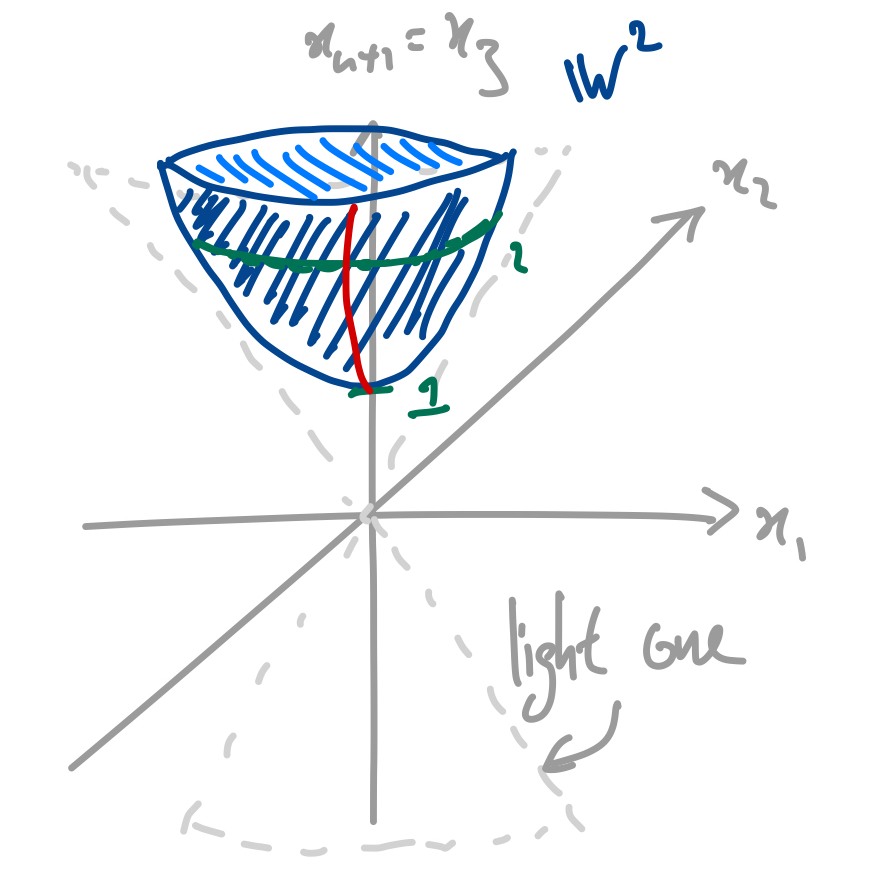
\includegraphics{hyperboloid}
      \caption{Illustration of the $\mathbb{W}^2$.}
      \label{fig:hyperboloid}
    \end{marginfigure}
    \begin{equation*}
      g_p(v, w) = \eta(v, w), \quad v,w \in T_p(\mathbb{W}^n).
    \end{equation*}
    For $n=2$, an almost global co-ordinate chart of $\mathbb{W}^2$ is given by
    \begin{align*}
      \phi^{-1} &: (0, 2\pi) \times (0,\infty) \to \mathbb{W}^2,\\
      (x_1, x_2) &\mapsto (\cos x_1 \sinh x_2, \sin x_1 \sinh x_2, \cosh x_2),
    \end{align*}
    since the image of $\phi^{-1}$ covers $\mathbb{W}^2$ except the curve obtained by intersection of $\mathbb{W}^2$ with the half-plane $\{x_1 \geq 0,\ x_2 = 0\}$. If we let $p = \phi^{-1}(x_1, x_2)$, then with the chart, we have
    \begin{align*}
      \left.\frac{\partial}{\partial x_1}\right|_p &= (-\sin x_1 \sinh x_2, \cos x_1 \sinh x_2, 0), \\
      \left.\frac{\partial}{\partial x_2}\right|_p &= (\cos x_1 \cosh x_2, \sin x_1 \cosh x_2, \sinh x_2),
    \end{align*}
    so that
    \begin{equation*}
      (g_{ij})(p) = \begin{pmatrix} g_{11} & g_{12} \\ g_{21} & g_{22} \end{pmatrix} = \begin{pmatrix} \sinh^2 x_2 & 0 \\ 0 & 1 \end{pmatrix},
    \end{equation*}
    so the metric is positive definite.
    
    \item \textbf{Poincar\'e's ball model}. Let $\mathbb{B}^n = \{p \in \mathbb{R}^n\ |\ \|p\|<1\}$ where $\|\cdot\|$ is the standard Eucliean norm. Since $\mathbb{B}^n \subset \mathbb{R}^n$ is open, the tangent space $T_p(\mathbb{B}^n)$ can be canonically identified with $\mathbb{R}^n$. The metric on this ball however we take to be
    \begin{equation*}
      g_p (v_1, v_2) = \frac{4}{(1-\|p\|^2)^2} \langle v_1, v_2 \rangle
    \end{equation*}
    where $\langle \cdot, \cdot\rangle$ is the standard Euclidean inner product. The distance gets progressively larger as we approach the boundary. See Fig.~\ref{fig:escher} for a rendering of $\mathbb{B}^2$, where we distance can be in units of fish, and the distance is increasingly stretched out as we approach the boundary of the disc.
    \begin{marginfigure}
      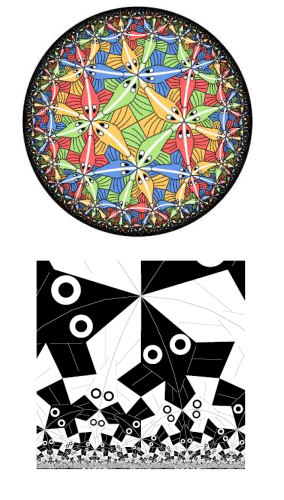
\includegraphics{escher}
      \caption{Computer rendering of M. C. Escher's \emph{Circle Limit III} and \emph{Circle Limit I}. From website of Douglas Dunham (UoM Duluth).}
      \label{fig:escher}
    \end{marginfigure}
    
    \item \textbf{Upper half plane model}. Similar to above, $\mathbb{H}^n = \{p \in \mathbb{R}^n\ |\ x_n > 0\}$. Again, $T_p(\mathbb{H}^n)$ can be identified with $\mathbb{R}^n$. The metric we choose here is
    \begin{equation*}
      g_p(v_1, v_2) = \frac{\langle v_1, v_2\rangle}{x_n^2},
    \end{equation*}
    and distance is increasingly stretched out as we approach the boundary of the half-plane; see Fig.~\ref{fig:escher} for a rendering of $\mathbb{H}^2$.
  \end{enumerate}
\end{example}

Let $V_{1,2}$ be two vector spaces with inner products $\langle\cdot,\cdot\rangle_{1,2}$. An isomorphism $T: V_1 \to V_2$ is called a \textbf{linear isometry} if
\begin{equation}
  \langle v_1, v_2 \rangle_1 = \langle T(v_1), T(v_2) \rangle_2
\end{equation}
for all $v_{1,2} \in V_1$.

Let $(M_1, g_1)$ and $(M_2, g_2)$ be two Riemannian manifolds. A bijective differentiable map $f: M_1 \to M_2$ with differentiable inverse $f^{-1}: M_2 \to M_1$ is called a \textbf{diffeomorphism}. A diffeomorphism $f$ above is called an \textbf{isometry} if $Df(p) : T_p(M_1) \to T_{f(p)}(M_2)$ is a linear isometry, i.e.
\begin{equation}
  \langle (Df(p))(v), (Df(p))(w)\rangle_{2, f(p)} = \langle v,w\rangle_{1, p}
\end{equation}
for all $v,w \in T_p(M_1)$.

\begin{remark}
  It is in face sufficient to check this for $v=w$, since
  \begin{equation*}
    \langle v,w\rangle_p = \frac{1}{4}\left(\|v+w\|^2_p - \|v-w\|^2_p\right).
  \end{equation*}
\end{remark}

\begin{example}
  \begin{enumerate}
    \item Let $f: \mathbb{W}^2 \to \mathbb{B}^2$ as above. We can map each point $p$ on the hyperboloid onto the a point on the disk that intersects the straight line through $p$ and $(0,0,-1)$ (e.g. the trough at $(0,0,1) \in \mathbb{W}^2$ is mapped to the origin), and vice-versa. Can do it in a way that preserves the inner product, so is an isometry.
    
    \item For $\mathbb{B}^2, \mathbb{H}^2 \subset \mathbb{R}^2 \cong \mathbb{C}$, we can show that
    \begin{equation*}
      f: \mathbb{H}^2 \to \mathbb{B}^2, \quad f(z) = \frac{z-\mathrm{i}}{z+\mathrm{i}}
    \end{equation*}
    is an isometry.\marginnote{Note that this $f$ is a M\"obius map.} We see that $f$ is a diffeomorphism with
    \begin{equation*}
      f^{-1} = \frac{z+1}{\mathrm{i}z - \mathrm{i}}.
    \end{equation*}
    Let $z=x+\mathrm{i}y \in \mathbb{H}^2$, $v = v_1 + \mathrm{i}v_2 \in T_z(\mathbb{H}^2)$. Then
    \begin{equation*}
      g_z^{\mathbb{H}^2}(v, v) = \frac{v_1^2 + v_2^2}{y^2}.
    \end{equation*}
    Let $c(t) = z + tv$ represent $v$, namely $c(0) = z$, $c'(0) = v$, so
    \begin{align*}
      (Df(z))(v) = (f\circ c)'(0)
        &= \left.\frac{\mathrm{d}}{\mathrm{d}t}\right|_{t=0} \left(\frac{c(t) - \mathrm{i}}{c(t) + \mathrm{i}}\right)\\
        &= \frac{c'(0)(z+\mathrm{i}) - c'(0)(z-\mathrm{i})}{(z+\mathrm{i})^2}\\
        &= \frac{2\mathrm{i}}{(z+1)^2}v \in T_z(\mathbb{B}^2).
    \end{align*}
    Here,
    \begin{equation*}
      g_z^{\mathbb{B}^2}(w, w)
        = \frac{4\left|\cfrac{2\mathrm{i}}{(z+1)^2}\right|^2}{\left(1-\left|\cfrac{z-\mathrm{i}}{z+\mathrm{i}}\right|^2\right)^2}\langle v,v\rangle 
        = \frac{16\langle v,v\rangle}{(|z+\mathrm{i}|^2 - |z-\mathrm{i}|^2)^2} = \frac{\langle v,v\rangle}{y^2},
    \end{equation*}
    and hence $f$ is an isometry.
  \end{enumerate}
\end{example}

\begin{lemma}
  Let $(M_1, g_1)$ and $(M_2, g_2)$ be two Riemannian manifolds and $f: M_1 \to M_2$ a diffeomorphism. Let $\phi: M_1 \to V \subset \mathbb{R}^n$ be a global co-ordinate chart with $\phi = (x_1, \ldots x_n)$, then $\psi = \phi \circ f^{-1} : M_2 \to V$ is a global co-ordinate chart of $M_2$. For $\psi = (y_1, \ldots y_n)$, i.e. $y_i = x_i \circ f$, $f$ is an isometry if
  \begin{equation*}
    \left\langle \left.\frac{\partial}{\partial x_i}\right|_p, \left.\frac{\partial}{\partial x_j}\right|_p \right\rangle_{1,p} = \left\langle \left.\frac{\partial}{\partial y_i}\right|_{f(p)}, \left.\frac{\partial}{\partial y_j}\right|_{f(p)} \right\rangle_{2, f(p)}
  \end{equation*}
  for all $p \in M_1$.
\end{lemma}

\begin{proof}
  First of all, we have
  \begin{equation*}
    (Df(p))\left(\left.\frac{\partial}{\partial x_i}\right|_p\right)(h) = \left.\frac{\partial}{\partial x_i}\right|_p (h\circ f) = \frac{\partial (h\circ f\phi^{-1})}{\partial x_i}(\phi(p)).
  \end{equation*}
  Noting that we have
  \begin{equation*}
    f\circ \phi^{-1} = \psi^{-1}, \quad \psi(f(p)) = \phi\circ f^{-1}(f(p)) = \phi(p),
  \end{equation*}
  then
  \begin{equation*}
    (Df(p))\left(\left.\frac{\partial}{\partial x_i}\right|_p\right)(h) = \frac{\partial (h\circ \psi^{-1})}{\partial x_i}(\psi(f(p))) = \left.\frac{\partial}{\partial y_i}\right|_{f(p)}.
  \end{equation*}
  $h$ is arbitrary, so
  \begin{equation*}
    (Df(p))\left(\left.\frac{\partial}{\partial x_i}\right|_p\right) = \left.\frac{\partial}{\partial y_i}\right|_{f(p)}.
  \end{equation*}
  
  Now, assuming that
  \begin{equation*}
    \left\langle \left.\frac{\partial}{\partial x_i}\right|_p, \left.\frac{\partial}{\partial x_j}\right|_p \right\rangle_{1,p} = \left\langle \left.\frac{\partial}{\partial y_i}\right|_{f(p)}, \left.\frac{\partial}{\partial y_j}\right|_{f(p)} \right\rangle_{2, f(p)}
  \end{equation*}
  Let $v \in T_p(M_1)$, then
  \begin{equation*}
    v = a_i \left.\frac{\partial}{\partial x_i}\right|_p \quad \Rightarrow \quad Df(p)(v) = a_i \left.\frac{\partial}{\partial y_i}\right|_{f(p)},
  \end{equation*}
  which implies
  \begin{align*}
    \langle Df(p)(v), Df(p)(v)\rangle_{2, f(p)} 
      &= \left\langle a_i \left.\frac{\partial}{\partial y_i}\right|_{f(p)}, a_j \left.\frac{\partial}{\partial y_j}\right|_{f(p)}\right\rangle_{2, f(p)}\\
      &= a_i a_j\left\langle \left.\frac{\partial}{\partial y_i}\right|_{f(p)}, \left.\frac{\partial}{\partial y_j}\right|_{f(p)}\right\rangle_{2, f(p)}\\
      &= a_i a_j\left\langle \left.\frac{\partial}{\partial x_i}\right|_p, \left.\frac{\partial}{\partial x_j}\right|_p\right\rangle_{1, p}\\
      &= \left\langle a_i \left.\frac{\partial}{\partial x_i}\right|_p, a_j\left.\frac{\partial}{\partial x_j}\right|_p\right\rangle_{1, p}\\
      &= \langle v, v\rangle_{1, p},
  \end{align*}
  and hence $Df(p)$ is a linear isometry and so $f$ is an isometry. \qed
\end{proof}

%-------------------------------------------------------------------------------

\section{Integration on Riemannian manifolds}

Let $(M,g)$ be a $n$-Riemannanian manifold and $\phi = (x_1, \ldots x_n) : U \to V \subset \mathbb{R}^n$ be a co-ordinate chart. Recall that
\begin{equation*}
  g_{ij}(p) = \left\langle \left.\frac{\partial}{\partial x_i}\right|_p, \left.\frac{\partial}{\partial x_j}\right|_p\right\rangle : U \to \mathbb{R}, \quad 1\leq i,j\leq n.
\end{equation*}
Let $f: M \to \mathbb{R}$ be a function with support in $U$ only, and $\phi$ as above. Then we define the integral to be
\begin{equation}
  \highlight{\int_M f\; \mathrm{d}(\mbox{vol}) = \int_U f\; \mathrm{d}(\mbox{vol}) = \int_V \left(f\circ \phi^{-1}\right)(x) \cdot \sqrt{\mbox{det}(g_{ij} \circ \phi^{-1}(x)}\; \mathrm{d}x}.
\end{equation}

To show that this definition is co-ordinate independent, let $F = \psi \circ \psi^{-1}$, $\psi = (y_1, \ldots y_n) : U \to V'$ be another co-ordinate chart, so $F$ is the change of co-ordinates. The transformation rule states that if $F: V \to V'$ is a diffeomorphism, then we need a Jacobian factor for the integral as
\begin{equation}
  \int_V' h(y)\; \mathrm{d}y = \int_V (h\circ F)(x) |\mbox{det}DF(x)|\; \mathrm{d}x.
\end{equation}
for some function $h$. Recall that
\begin{equation*}
  \left.\frac{\partial}{\partial x_i}\right|_p = \frac{\partial y_j}{\partial x_i}(p)\left.\frac{\partial}{\partial y_j}\right|_p,
\end{equation*}
so the metric is
\begin{align*}
  \tilde{g}_{ij}(p) 
    &= \left\langle \left.\frac{\partial}{\partial x_i}\right|_p, \left.\frac{\partial}{\partial x_j}\right|_p\right\rangle\\
    &=\frac{\partial y_k}{\partial x_i}(p) \frac{\partial y_l}{\partial x_i}(p) \left\langle \left.\frac{\partial}{\partial y_k}\right|_p, \left.\frac{\partial}{\partial y_l}\right|_p\right\rangle\\
    &=\left(\frac{\partial y_k}{\partial x_i}(p)\right)(g_{kl}'(p)) \left(\frac{\partial y_l}{\partial x_j}(p)\right)^T
\end{align*}
for $p\in M$, where $g_{kl}'$ is the metric expressed in the $y$ co-ordinates. Let $x = \phi(p)$, then since $F_j = y_j \circ \phi^{-1}$, we have
\begin{equation*}
  DF(x) = \left(\frac{\partial (y_i \circ \phi^{-1})}{\partial x_j}(x)\right) = \left(\frac{\partial y_i}{\partial x_j}(p)\right),
\end{equation*}
so then $(g_{ij}(p)) = (DF(x))^T (g'_{ij}(p)) (DF(x))$, and since the transpose does not alter the determinant,
\begin{equation*}
  \sqrt{\mbox{det}g_{ij}(p)} = |\mbox{det}DF| \sqrt{\mbox{det}g_{ij}'(p)}.
\end{equation*}
Thus
\begin{equation*}
  \int_V (f\circ \phi^{-1})\sqrt{\mbox{det}(g_{ij} \circ \phi^{-1})}\; \mathrm{d}x = \int_V (f\circ \psi^{-1} \circ F)\sqrt{\mbox{det}(g'_{ij} \circ \psi^{-1} \circ F)} |\mbox{det}DF|\; \mathrm{d}x.
\end{equation*}
If we then define the function $h$ above to be $h = f \circ \psi^{-1}\sqrt{\mbox{det}(g_{ij}'\circ \psi^{-1})}$, then by the transformation rule we have that
\begin{equation*}
  \int_V (f\circ \phi^{-1})\sqrt{\mbox{det}(g_{ij} \circ \phi^{-1})}\; \mathrm{d}x = \int_{V'} (f\circ \psi^{-1})\sqrt{\mbox{det}(g_{ij}' \circ \psi^{-1})}\; \mathrm{d}y,
\end{equation*}
and we have co-ordinate independence as claimed.

Let $(M,g)$ be a Riemanninan manifold with a global co-orindate chart $\phi = (x_1, \ldots x_n) : M \to \mathbb{R}^n$. The \textbf{volume} of $A \subset M$ is
\begin{equation}
  \highlight{\mbox{vol}(A) = \int_M \mathbb{1}_A\; \mathrm{d}(\mbox{vol}) = \int_A\; \mathrm{d}(\mbox{vol} = \int_{\phi(A)}\sqrt{\mbox{det}(g_{ij} \circ \phi^{-1})}\; \mathrm{d}x},
\end{equation}
where $\mathbb{1}_A$ is the indicator function supported over $A$.

\begin{example}
  Recall that $\mathbb{H}^2 = \{z\ |\ \mbox{Im}(z)>0\}$ with $\langle v,w\rangle = (v_1 w_1 + v_2 w_2) / y^2$ for $z=x+\mathrm{i}y$ has the global chart $\phi : \mathbb{H}^2 \to \mathbb{R}^2$ with $x+\mbox{i}y \mapsto (x,y)$. Then
  \begin{align*}
      g_{11}(z) = \left\langle \left.\frac{\partial}{\partial x_1}\right|_z, \left.\frac{\partial}{\partial x_1}\right|_z \right\rangle = \frac{1}{y^2} = g_{22}(z),\quad g_{12}(z) = g_{21}(z) = 0.
  \end{align*}
  For what would be visually the rectangular strip $A = \{z\in \mathbb{H}^2\ |\ 0 < a \leq y \leq b,\ -n \leq x \leq n\}$, we would have
  \begin{equation*}
    \mbox{vol}(A) = \int_{-n}^n \int_a^b \sqrt{\mbox{det}g_{ij}}\; \mathrm{d}y\; \mathrm{d}x = 2n\left(\frac{1}{a} - \frac{1}{b}\right),
  \end{equation*}
  as opposed to $2n(b-a)$ under the usual metric.
\end{example}

Let $M$ be a differentiable manifold. A \textbf{partition of unity} on $M$ is some $\{\psi_\alpha \in C^\infty(M)\}_{\alpha\in A}$, $\psi_\alpha : M \to [0, 1]$ such that
\begin{itemize}
  \item for all $p\in M$, there exists an open neighbourhood $U_p \subset M$ with $\left.\psi_\alpha\right|_{U_p} \neq 0$ for finite many $\alpha \in A$,
  \item $\sum_{\alpha \in A} \psi_\alpha = 1$.
\end{itemize}
Let $\{U_\alpha\}_{\alpha \in A}$ be an open cover of $M$. A partition of unity $\{\psi_\alpha\}_{\alpha \in A}$ is \textbf{subordinated} to $\{U_\alpha\}$ if, for all $\alpha \in A$, $\mbox{supp} \psi_\alpha \subset U_\alpha$.\marginnote{$\mbox{supp}$ is support rather than supremum.}

\begin{theorem}
  Let $M$ be a manifold and $\{U_\alpha, \phi_\alpha\}_{\alpha \in A}$ be a countable atlas of $M$. Then there exists a partition of unity $\{\psi_\alpha\}$ subordinated to $\{U_\alpha\}$. \qedwhite
\end{theorem}

Let $(M,g)$ be a Riemannian manifold with countable atlas $\{U_\alpha, \phi_\alpha\}_{\alpha \in A}$ and subordinated partition of unity $\{\psi_\alpha\}$. For any $f: M\to \mathbb{R}$, we define the \textbf{integral} of $f$ as
\begin{equation}
  \highlight{\int_M f\; \mathrm{d}(\mbox{vol}) = \sum_{\alpha \in A} \int_M f\psi_\alpha\; \mathrm{d}(\mbox{vol})}.
\end{equation}
This definition is independent of atlas and partition of unity.

%-------------------------------------------------------------------------------

\section{Riemannian manifolds as metric spaces}

Let $(M,g)$ be a Riemannian manifold, $c:[a,b] \to M$ be a differentiable curve. The \textbf{length} of $c$ is
\begin{equation}
  \highlight{L(c) = \int_a^b \|c'(t)\|_{c(t)}\; \mathrm{d}t}.
\end{equation}
If $c$ is piecewise smooth with cusps, then just chop it up in the the bits that can be integrated accordingly and then sum it up, i.e.
\begin{equation}
  L(c) = \sum_{i=0}^{n-1} \int_{t_i}^{t_{i+1}} \|c'(t)\|_{c(t)}\; \mathrm{d}t.
\end{equation}

\begin{theorem}
  Let $c: [0,T] \to M$ be a differentiable curve and $\gamma : [0, S]$ be an orientation preserving re-parameterisation of $c$ (i.e. there exists a strictly monotonic differentiable function $\phi:[0,T] \to [0,S]$ with $\phi(0)=0$, $\phi(T) = S$ such that $\gamma = c\circ \phi$. Then $L(c) = L(\gamma)$.
\end{theorem}

\begin{proof}
  For $f \in D(M, \gamma(s))$,
  \begin{equation*}
    \gamma'(s)(f) = (f\circ \gamma)'(s) = (f\circ c\circ \phi)'(s).
  \end{equation*}
  By the chain rule, we have
  \begin{equation*}
    (f\circ c\circ \phi)'(s) = (f\circ c)'(\phi(s))\cdot \phi'(s) = \phi'(s)c'(\phi(s))(f)
  \end{equation*}
  so that $\phi'(s) c'(\phi(s)) = \gamma'(s)$. Since $\phi$ was assumed to be orientation preserving and monotonic,
  \begin{align*}
    L(\gamma) 
      &= \int_0^S \|\gamma'(s)\|_{\gamma(s)}\; \mathrm{d}s \\
      &= \int_0^S \phi'(s)\|c'(\phi(s))\|_{c(\phi(s))}\; \mathrm{d}s \\
      &= \int_0^T \|c'(t)\|_{c(t)}\; \mathrm{d}s = L(c)
  \end{align*}
  since $t = \phi(s)$. \qed
\end{proof}
Note the result is true even if re-parameterisation is orientation reversing, as there will be two minus signs arising in that case.

A differentiable curve $c: [a,b] \to M$ is \textbf{parameterised by arc length} if $\|c'(t)\|_{c(t)} = 1$ for all $t \in [a,b]$.

\begin{lemma}
  For an arc length parameterised curve $c:[a,b] \to M$, $L(c|_{[a,t]}) = t-a$ for all $t\in [a,b]$. (Just use the definition.) \qedwhite
\end{lemma}

\begin{proposition}
  Every differentiable curve $c:[a,b] \to M$ with $c'(t) \neq 0$ for all $t\in [a,b]$ has an arc length re-parameterisation $\gamma : [0, L(\gamma)] \to M$.
\end{proposition}

\begin{proof}
  Let $\ell : [a,b] \to [0, L(\gamma)]$, $\ell(t) = L(c|_{[a,t]}) = \int_a^t \|c'(s)\|_{c(s)}\; \mathrm{d}s$. Clearly $\ell$ is differentiable and $\ell'(t) = \|c'(t)\|_{c(t)} > 0$, so $\ell$ is strictly monotonically increasing and hence bijective. Since $\ell(\ell^{-1}(s)) = s$,
  \begin{equation*}
    \ell'(\ell^{-1}(s))\cdot (\ell^{-1})'(s) = 1,
  \end{equation*}
  which implies
  \begin{equation*}
   (\ell^{-1})'(s) = \frac{1}{\|c'(\ell^{-1}(s))\|_{c(\ell^{-1}(s))}}.
  \end{equation*}
  Let $\gamma = c \circ \ell^{-1} : [0, L(\gamma)] \to M$, then
  \begin{equation*}
    \|\gamma'(s)\| = (\ell^{-1})'(s) \|c'(\ell^{-1}(s))\|_{\ell(\ell^{-1}(s))} = 1,
  \end{equation*}
  and hence we have an arc length re-parameterisation.
\end{proof}

\begin{example}
  For $c : [a,b] \to \mathbb{H}^2$,  $c(t) = \mathrm{i}t$, then
  \begin{equation*}
    L(c) = \int_a^b \|c'(t)\|_{c(t)}\; \mathrm{d}t = \int_a^b \frac{|\mathrm{i}|}{t}\; \mathrm{d}t = \log \frac{b}{a}.
  \end{equation*}
  We show that for any other curve $\gamma:[0,T] \to \mathbb{H}^2$ with $\gamma(0)=a\mathrm{i}$, $\gamma(T)=b\mathrm{i}$, $L(\gamma) \geq L(c)$.\marginnote{This is related to the fact this $c(t)$ is a \textbf{geodesic} in $\mathbb{H}^2$, and has the property that it is distance minimising.} Let $\gamma(t) = x(t) + \mathrm{i}y(t)$, then since $y(t)>0$,
  \begin{align*}
    L(\gamma) = \int_0^T \|\gamma'(t)\|_{\gamma(t)}\; \mathrm{d}t
      &= \int_0^T \frac{\sqrt{(x')^2 + (y')^2}}{y}\; \mathrm{d}t\\
      &\geq \int_0^T \frac{\sqrt{(y')^2}}{y}\; \mathrm{d}t = \int_0^T \frac{|y'|}{y}\; \mathrm{d}t\\
      &\geq \int_0^T \frac{y'}{y}\; \mathrm{d}t = \log \frac{y(T)}{y(0)} = \log \frac{b}{a} = L(c).
  \end{align*}
\end{example}

Let $(M,g)$ be a connected Riemannian manifold (i.e. for every $p,q\in M$, there is some $c : [a,b] \to M$ with $c(a)=p$, $c(b)=q$. We define a \textbf{distance function} $d_g : M\times M \to [0, \infty)$ as
\begin{equation}
  d_g(p,q) = \inf\{ L(c)\ |\ c\textnormal{ piecewise differentiable},\ c(a) = p,\ c(b) = q\}.
\end{equation}
The distance function should satisfy
\begin{itemize}
  \item $d_g(p,q) = 0$ iff $p=q$
  \item $d_g(p,q) = d(q,p)$
  \item $d_g(p_1, p_3) \leq d_g(p_1, p_2) + d_g(p_2, p_3)$
\end{itemize}
For a space equipped with a distance function $d_g$, $(X,d)$ is called a \textbf{metric space}.

\begin{example}
  Let $M = \mathbb{R}^2 \setminus \{0\}$ equipped with the standard Riemannian metric. Taking two points $p$ and $q=-p$, we see there is no curve $c:[a,b]\to \mathbb{R}^2\{0\}$ such that $L(c) = d_g(q-p)$ since such a curve passes through zero, which is not in the manifold.
\end{example}

Give $c:[a,b] \to M$ with $L(c) = d_g(c(a), c(b))$, $c$ is called a \textbf{distance realising} curve.

Let $(X, d)$ be a metric space. A subset $A \subset X$ is called \textbf{compact} if for all sequence $(x_n)_{n\in\mathbb{N}} \in A$, there is a sub-sequence $(x_{n_j})_{j\in\mathbb{N}}$ such that $d(x_{n_j}, x_\infty) \to 0$ as $j\to\infty$. The metric space here is \textbf{complete} if every Cauchy sequence in $X$ is convergent, i.e. for all $(x_n)_{n\in\mathbb{N}} \in X$ and $\epsilon>0$, there exists some $N$ where $d(x_n, x_m) < \epsilon$ for all $n,m\in\mathbb{N}$, with limit point $x_\infty \in X$ where $d(x_n, x_\infty)\to 0$.

\begin{example}
  $\mathbb{R} \setminus \{0\}$ is not complete since $(1/n)_{n\in \mathbb{N}}$ is a Cauchy sequence but its limit is not in the space.
\end{example}

%===============================================================================

\chapter{Levi-Civita connection and parallel transport}

We aim to differentiate a vector field $X: M\to T(M)$ along a curve $c$. As an example, we consider directional derivatives of a vector field in $\mathbb{R}^n$. By identifying $T_p(\mathbb{R}^n) \cong \mathbb{R}^n$, a vector field of $X$ on $\mathbb{R}^n$ can be considered as a map $X:\mathbb{R}^n \to \mathbb{R}^n$, i.e. $X = a_i(\partial / \partial x_i)$, so
\begin{equation*}
  X(p) = a_i(p) \left.\frac{\partial}{\partial x_i}\right|_p \cong (a_i(p))_i \in \mathbb{R}^n.
\end{equation*}
For a tangent vector $v \in T_p(\mathbb{R}^n)$, we can naturally define the derivative of $x$ in the direction of $v$ by
\begin{equation}
  \highlight{\nabla_v X = v(a_j)(\partial / \partial x_j)|_p},
\end{equation}
since
\begin{align*}
  \nabla_v X = DX(p)(v) 
    &= \lim_{t\to 0} \frac{X(p+tv) - X(p)}{t} \\
    &= \left(\lim_{t\to 0} \frac{a_i(p+tv) - a_i(p)}{t}\right)_i\\
    &= (v(a_i))_i \\
    &= v(a_j)\boldsymbol{e}_j \\
    &= v(a_j) \left.\frac{\partial}{\partial x_j}\right|_p.
\end{align*}
Here, $\nabla_v X \in T_p(\mathbb{R}^n)$ is called the \textbf{covariant derivative} of $X$ in the direction of $v$. Note that we define $\nabla_X Y \in \mathcal{X}(\mathbb{R}^n)$, with
\begin{equation}
  \highlight{\nabla_X Y(p) = \nabla_{X(p)}Y(p) \in T_p(\mathbb{R}^n)}.
\end{equation}
The \textbf{torsion} is defined as
\begin{equation}
  \highlight{T(X,Y) = \nabla_X Y - \nabla_Y X -  [X, Y]},
\end{equation}
and described how tangent spaces twist around a curve.

\begin{proposition}
  For $X,Y: \to \mathbb{R}^n \to \mathbb{R}^n$, $v,w\in T_p(\mathbb{R}^n)$, $\alpha,\beta\in \mathbb{R}$, $f\in C^\infty(\mathbb{R}^n)$, we have
  \begin{enumerate}
    \item linearity in vector field, $\nabla_v (X+Y) = \nabla_v X + \nabla_v Y$
    \item product rule, $\nabla_v (fX) = v(f)\cdot X(p) + f(p)\nabla_v X$
    \item linearity in directional vector, $\nabla_{\alpha v+\beta w} X = \alpha \nabla_v X + \beta\nabla_w X$
    \item Riemannian property, $v(\langle X, Y\rangle) = \langle \nabla_v X, Y(p)\rangle + \langle X(p), \nabla_v Y\rangle$
    \item torsion freeness, $\nabla_X Y - \nabla_Y X = [X, Y]$.
  \end{enumerate}
\end{proposition}

\begin{proof}
  \begin{enumerate}
    \item For $X = (a_i)_i$, $Y = (b_i)_i$,
    \begin{equation*}
      \nabla_v (X+Y) = v(a_i + b_i)\boldsymbol{e}_i = v(a_i)\boldsymbol{e}_i + v(b_i)\boldsymbol{e}_i = \nabla_v X + \nabla_v Y.
    \end{equation*}
    
    \item As above,
    \begin{align*}
      \nabla_v(fX) = v(fa_i)\boldsymbol{e}_i 
        &= v(f)a_i(p)\boldsymbol{e}_i + f(p)v(a_i)\boldsymbol{e}_i\\
        &= v(f) X(p) + f(p) \nabla_v X.
    \end{align*}
    
    \item Also as above,
    \begin{align*}
      \nabla_{\alpha v+\beta w} X = (\alpha v + \beta w)a_i\boldsymbol{e}_i
        &= \alpha v(a_i)\boldsymbol{e}_i + \beta w(a_i)\boldsymbol{e}_i\\
        &= \alpha \nabla_v X + \beta \nabla_w Y.
    \end{align*}
    
    \item For $\langle X, Y\rangle = a_i b_i$, we have
    \begin{equation*}
      \langle \nabla_v X, Y(p)\rangle = \langle v(a_i)\boldsymbol{e}_i, b_j(p)\boldsymbol{e}_j \rangle = v(a_i) b_i(p).
    \end{equation*}
    Similarly, we have
    \begin{equation*}
      \langle \nabla_v X(p), \nabla_v Y\rangle = v(b_i) a_i(p),
    \end{equation*}
    so their sum would be
    \begin{equation*}
      v(a_i) b_i(p) + v(b_i)a_i(p) = v(a_i b_i)(p) = v\langle X(p), Y(p)\rangle.
    \end{equation*}
    
    \item We have
    \begin{equation*}
      (\nabla_X Y)(p) = X(p)(b_i)\boldsymbol{e}_i = a_j(p) \frac{\partial b_i}{\partial x_j}(p)\left.\frac{\partial}{\partial x_i}\right|_p,
    \end{equation*}
    while
    \begin{equation*}
      (\nabla_Y X)(p) = Y(p)(a_i)\boldsymbol{e}_i = b_j(p) \frac{\partial a_i}{\partial x_j}(p)\left.\frac{\partial}{\partial x_i}\right|_p,
    \end{equation*}
    so
    \begin{align*}
      (\nabla_X Y)(p) - (\nabla_Y X)(p) 
        &= \left(a_j(p) \frac{\partial b_i}{\partial x_j}(p) - b_j(p) \frac{\partial a_i}{\partial x_j}(p)\right)\left.\frac{\partial}{\partial x_i}\right|_p\\
        &=[X, Y](p).
    \end{align*}
    \qed
  \end{enumerate}
\end{proof}

Since
\begin{equation*}
  (\nabla_X Y)(p) = \lim_{t\to 0}\frac{Y(p + tX(p)) - Y(p)}{t},
\end{equation*}
we also have the following:
\begin{enumerate}
  \item $\nabla_X (Y+Z) = \nabla_X Y +\nabla_X Z$,
  \item $\nabla_X (fY) = [X(f)]Y + f\nabla_X Y$,
  \item $\nabla_{fX + gY} Z = f \nabla_X Z + g\nabla_Y Z$,
  \item $X(\langle Y,Z\rangle) = \langle \nabla_X Y, Z\rangle + \langle Y, \nabla_X Z\rangle$,
  \item $\nabla_X Y - \nabla_Y X = [X, Y]$.
\end{enumerate}

Let $M$ be a differentiable manifold, and $\mathcal{X}(M)$ be the space of all vector fields on $M$. A map $\nabla: \mathcal{X}(M) \times \mathcal{X}(M) \to \mathcal{X}(M)$ satisfying the first three properties above is called an \textbf{covariant derivative} (or \textbf{affine connection}).\marginnote{An affine connection `connects' nearby tangent spaces, allowing the notion of derivative to make sense.}

\begin{theorem}[Fundamental theorem of Riemannian geometry]
  Let $(M,g)$ be a Riemannian manifold. Then there exists a unique covariant derivative $\nabla$ satisfying the Riemannian and torison freeness property (i.e. all properties above), and this connection is called the \textbf{Levi-Civita connection}.
\end{theorem}
  
\begin{proof}

  For uniqueness, note that since $\nabla$ is Riemannian, we have
  \begin{align*}
    X\langle Y,Z\rangle &= \langle \nabla_X Y, Z\rangle + \langle Y, \nabla_X Z\rangle,\\
    Y\langle Z,X\rangle &= \langle \nabla_Y Z, X\rangle + \langle Z, \nabla_Y X\rangle,\\
    Z\langle X,Y\rangle &= \langle \nabla_Z X, Y\rangle + \langle X, \nabla_Z Y\rangle,
  \end{align*}
  so that (with torsion freeness and properties of the inner product)
  \begin{align*}
    X\langle Y,Z\rangle + Y\langle Z,X\rangle - Z\langle X,Y\rangle
      &= \langle \nabla_X Y, Z\rangle + [\langle Y, \nabla_X Z\rangle - \langle \nabla_Z X, Y\rangle] \\
      +& [\langle \nabla_Y Z, X\rangle - \langle X, \nabla_Z Y\rangle] \\
      +& \langle Z, [Y,X] + \nabla_X Y\rangle\\
      &= \langle \nabla_X Y, Z\rangle + \langle Y, \nabla_X Z - \nabla_Z X\rangle\\
      +& \langle X, \nabla_Y Z - \nabla_Z Y\rangle\\
      +& \langle Z, [Y,X]\rangle + \langle Z, \nabla_X Y\rangle\\
      &= 2\langle \nabla_X Y, Z\rangle + \langle Y, [X,Z]\rangle\\
      +& \langle X, [Y,Z]\rangle + \langle Z, [Y,X]\rangle,
  \end{align*}
  which provides an explicit construction for $\nabla_X Y$ via
  \begin{equation}\begin{aligned}\label{eq:covariant}
    \langle \nabla_X Y, Z\rangle = 
      &\frac{1}{2}( X\langle Y, Z\rangle + Y\langle Z,X \rangle - Z\langle X,Y \rangle \\
      &-\langle Y, [X,Z]\rangle - \langle X, [Y,Z]\rangle - \langle Z, [Y,X]\rangle).
  \end{aligned}\end{equation}
  
  For existence, we check that the above construction satisfies the properties. Clearly we have linearity since the inner product and Lie bracket are linear. The expression above satisfies the product rule, torsion freeness and Riemannian property follows essentially by brute force calculation. \qed
\end{proof}

%-------------------------------------------------------------------------------

\section{Christoffel symbols}

Let $(M,g)$ be a Riemannian manifold, and $\nabla$ the Levi-Civita connection on $(M,g)$. For $\phi = (x_1, \ldots x_n): U\to V \subset \mathbb{R}^n$ a co-ordinate chart, we have
\begin{equation}
  \highlight{\left(\nabla_{\left.\frac{\partial}{\partial x_i}\right|_p} \frac{\partial}{\partial x_j}\right)(p) = \Gamma_{ij}^k \left.\frac{\partial}{\partial x_k}\right|_p},
\end{equation}
where $\Gamma{ij}^k : U\to\mathbb{R}$ are the \textbf{Christoffel symbols} of the covariant derivative with respect to $\phi$. Observing that $[\partial / \partial x_i, \partial / \partial x_j] = 0$, with Eq.~\eqref{eq:covariant},
\begin{align*}
  \left\langle \nabla_{\left.\frac{\partial}{\partial x_i}\right|_p} \frac{\partial}{\partial x_j}, \frac{\partial}{\partial x_l} \right\rangle(p)
    &= \frac{1}{2} \left[ \frac{\partial}{\partial x_i}\left\langle \frac{\partial}{\partial x_j}, \frac{\partial}{\partial x_l}\right\rangle + \frac{\partial}{\partial x_j}\left\langle \frac{\partial}{\partial x_i}, \frac{\partial}{\partial x_l}\right\rangle - \frac{\partial}{\partial x_l}\left\langle \frac{\partial}{\partial x_i}, \frac{\partial}{\partial x_j}\right\rangle \right](p)\\
    &= \frac{1}{2}(g_{jl,i} + g_{il,j} - g_{ij,l})(p)
\end{align*}
where $g_{jl,i} = \partial g_{jl} / \partial x_i$. Since $(g_{ij})$ is symmetric and invertible by construction, we denote the entries of $(g_{ij})^{-1}$ by $g^{ij}$, and we thus have the equation
\begin{equation*}
  \Gamma_{ij}^k g_{kl} = \frac{1}{2}(g_{jl,i} + g_{il,j} - g_{ij,l}),
\end{equation*}
so that
\begin{equation}
  \highlight{\Gamma_{ij}^k = \frac{1}{2}(g_{jl,i} + g_{il,j} - g_{ij,l})g^{kl}}.
\end{equation}

\begin{remark}
  \begin{itemize}
    \item $g_{lm} = g_{ml}$ implies that $g^{lm} = g^{ml}$.
    \item $\Gamma_{ij}^k = \Gamma_{ji}^k$ be the fact that $g_{ij}$ is symmetric.
  \end{itemize} 
\end{remark}

\begin{example}
  Recall that for $\mathbb{H}^2$ we have $\langle v,w\rangle_z = \langle v, w\rangle / y^2$, $z=x + \mathrm{i}y$, and that
  \begin{equation*}
    g_{ij}(z) = \frac{1}{y^2}I \quad \Rightarrow \quad g^{ij}(z) = y^2 I.
  \end{equation*}
  The metric has no off-diagonal terms, and any $g_{ij,1}$ is going to be zero since there is no $x$ dependence. For example,
  \begin{align*}
    \Gamma_{11}^1 &= \frac{1}{2}(g_{1l,1} + g_{1l,1} - g_{11,l})g^{l1} &= \frac{1}{2}(g_{11,1} + g_{11,1} - g_{11,1})g^{11} &= 0,\\
    \Gamma_{11}^2 &= \frac{1}{2}(g_{1l,1} + g_{1l,1} - g_{11,l})g^{l2} &= \frac{1}{2}(g_{12,1} + g_{12,1} - g_{11,2})g^{22} &= -\frac{1}{2}\left(-2\frac{1}{y^3}\right)y^2 = \frac{1}{y}
  \end{align*}
  and so forth. To summarise, there should be eight entries, and
  \begin{equation*}
    \Gamma_{11}^1 = \Gamma_{12}^2 = \Gamma_{21}^2 = \Gamma_{22}^1 = 0, \quad
   -\Gamma_{11}^2 = \Gamma_{12}^1 = \Gamma_{21}^1 = \Gamma_{22}^2 = -\frac{1}{y}. 
  \end{equation*}
  Then note that
  \begin{align*}
    \nabla_{\frac{\partial}{\partial x}}\frac{\partial}{\partial x} &= \Gamma_{11}^1 \frac{\partial}{\partial x} + \Gamma_{11}^2 \frac{\partial}{\partial y} = +\frac{1}{y}\frac{\partial}{\partial y} \\
    \nabla_{\frac{\partial}{\partial y}}\frac{\partial}{\partial y} &= \Gamma_{22}^1 \frac{\partial}{\partial x} + \Gamma_{22}^2 \frac{\partial}{\partial y} = -\frac{1}{y}\frac{\partial}{\partial y},
  \end{align*}
  while by the torison-free property and that $[\partial / \partial x, \partial / \partial y] = 0$,
  \begin{align*}
    \nabla_{\frac{\partial}{\partial x}}\frac{\partial}{\partial y} &= \Gamma_{12}^1 \frac{\partial}{\partial x} + \Gamma_{12}^2 \frac{\partial}{\partial y} = -\frac{1}{y}\frac{\partial}{\partial x} \\
    \nabla_{\frac{\partial}{\partial y}}\frac{\partial}{\partial x} &= \left[\frac{\partial}{\partial y}, \frac{\partial}{\partial x}\right] + \nabla_{\frac{\partial}{\partial y}}\frac{\partial}{\partial x} =-\frac{1}{y}\frac{\partial}{\partial x}.
  \end{align*}
  
  Let $X(z) = y(\partial / \partial y)|_z$ be a vector field (and note that $\|X(z)\|_z = 1$ in the present metric). We have
  \begin{align*}
    (\nabla_X X)(z) 
      &= y\left( \nabla_{\frac{\partial}{\partial y}} \left( y\frac{\partial}{\partial y} \right) \right)(z)\\
      &= y\left[\frac{\partial y}{\partial y}\frac{\partial}{\partial y} + y \nabla_{\frac{\partial}{\partial y}} \frac{\partial}{\partial y} \right](z)\\
      &= y\left( 1\frac{\partial}{\partial y} - y \frac{1}{y}\frac{\partial}{\partial y}\right)(z) = 0.
  \end{align*}
  The covariant derivative of $X$ in the direction $X$ vanishes, which is perhaps not that surprising.
\end{example}

%-------------------------------------------------------------------------------

\section{Parallel transport}

Let $(M,g)$ be a Riemannian manifold, $\nabla$ the Levi-Civita connection, $c[a,b] \to M$ a curve, $X \in \mathcal{X}(M)$, then $\nabla_{c'(t)} X \in T_{c(t)}(M)$ only depends on $X$ along $c$, i.e. if $\tilde{X} \in \mathcal{X}(M)$ with $\tilde{X}(c(t)) = X(c(t))$ for all $t \in [a,b]$ then $\nabla_{c'(t)}X = \nabla_{c'(t)} \tilde{X}$.

Let $c:[a,b] \to M$ be a differentiable curve on a Riemannian manifold. A map $X:[a,b] \to T(M)$ with $X(t) \in T_{c(t)}(M)$ is called a \textbf{vector field along $c$}. The space of all such vector fields is denoted by $\mathcal{X}_c(M)$.

\begin{example}
  For $c:[a,b] \to M$ a curve, then $t\mapsto c'(t)$ is a vector field along $c$.
\end{example}

\begin{proposition}
  Let $\nabla$ be the Levi-Civita connection of $(M,g)$, $c:[a,b] \to M$ a curve. Then there is a unique map called the \textbf{covariant derivative} along $c$
  \begin{equation}
    \frac{\mathrm{D}}{\mathrm{d}t} : \mathcal{X}_c(M) \to \mathcal{X}_c(M)
  \end{equation}
  satisfying
  \begin{enumerate}
    \item $(\mathrm{D} / \mathrm{d}t) (aX + bY) = a (\mathrm{D}X / \mathrm{d}t) + b (\mathrm{D}Y / \mathrm{d}t)$ for $a,b\in \mathbb{R}$,
    \item $(\mathrm{D} / \mathrm{d}t) (fX) = f'X + f (\mathrm{D}X / \mathrm{d}t)$ for $f\in C^\infty([a,b])$,
    \item for $\tilde{X} \in \mathcal{X}(M)$ a local extension of $X$, i.e. there exists $t_0 \in[a,b]$ where $\tilde{X}(c(t)) = X(t)$ for all $t \in [t_0 - \epsilon, t_0 + \epsilon]$ for some $\epsilon > 0$, we have
    \begin{equation}
      \frac{\mathrm{D}X}{\mathrm{d}t}(t_0) = \nabla_{c'(t_0)} \tilde{X}.
    \end{equation}
  \end{enumerate}
\end{proposition}

\begin{proof}
  To proof uniqueness, let $\phi = (x_1, \ldots x_n) : U \to V \subset \mathbb{R}^n$ be a co-ordinate chart with $c([t_0 - \epsilon, t_0 + \epsilon]) \subset U$, $X \in \mathcal{X}_c(M)$. Then, locally,
  \begin{equation*}
    X(t) = a_i(t) \left.\frac{\partial}{\partial x_i}\right|_{c(t)},
  \end{equation*}
  so that
  \begin{equation*}
    \frac{\mathrm{D}X}{\mathrm{d}t}(t) = a_i'(t) \left.\frac{\partial}{\partial x_i}\right|_{c(t)} + a_i(t) \frac{\mathrm{D}}{\mathrm{d}t}\left(\frac{\partial}{\partial x_i} \circ c\right)(t).
  \end{equation*}
  Note that $(\partial / \partial x_i \circ c) \in \mathcal{X}_c(M)$ and is a natural extension of $X$, so
  \begin{equation*}
    \frac{\mathrm{D}X}{\mathrm{d}t}(t) = a_i'(t) \left.\frac{\partial}{\partial x_i}\right|_{c(t)} + a_i(t) \nabla_{c'(t)} \frac{\partial}{\partial x_i} \in T_{c(t)}(M),
  \end{equation*}
  and hence we have uniqueness. Since above is an explicit construction, we can check that it satisfies all the desired properties, so we also have existence. \qed
\end{proof}

\begin{example}
  Let $M\subset \mathbb{R}^3$ be a surface, $\mathrm{D}/\mathrm{d}t$ the covariant derivative along a curve $c$, and $X\in \mathcal{X}_c(t)$ with $X(t) = [a_i(t)]_i \in \mathbb{R}^3 \cong T_{c(t)}(\mathbb{R}^3)$. Then
  \begin{equation*}
    \frac{\mathrm{D}X}{\mathrm{d}t}(t) = \pi_{c(t)}[a_i'(t)]_i \in T_{c(t)}(M)
  \end{equation*}
  where $\pi_{c(t)}$ is the orthogonal projection onto $M$. In particular, if $c(t) \in M$, then $c(t) \in T_{c(t)}(M)$, and
  \begin{equation*}
    \frac{\mathrm{D}c'}{\mathrm{d}t}(t) = \pi_{c(t)}[c_i''(t)]_i.
  \end{equation*}
  For $\mathrm{D}c' / \mathrm{d}t \equiv 0$, this is equivalent to $c''(t)$ being normal to $T_{c(t)}(M)$.\marginnote{This is the condition revisited later that $c$ is a \textbf{geodesic}.}
\end{example}

A vector field $X:[a,b] \to T(M)$ along $c$ is called \textbf{parallel along $c$} iff $\mathrm{D}X / \mathrm{d}t \equiv 0$.\marginnote{A geodesic is defined to be a curve whose tangent vectors remain parallel if they are transported along it. Requires the notion of an affine connection.}

\begin{theorem}
  Let $c:[a,b] \to M$ be a curve on a Riemannian manifold $(M,g)$ and $v\in T_{c(a)}(M)$. Then there exists a unique parallel vector field $X \in \mathcal{X}_c(M)$ with $X(a) = v$. Also, for $\mbox{dim}M = n$, the space of all parallel vector fields in $\mathcal{X}_c(M)$ is a $n$-vector space over $\mathbb{R}$.
\end{theorem}

\begin{proof}
  For simplicity, assume there exists a co-ordinate chart $\phi = (x_1, \ldots x_n): U\to V \subset \mathbb{R}^n$ with $c([a,b]) \subset U$. Let
  \begin{equation*}
     X(t) = a_i \left.\frac{\partial}{\partial x_i}\right|_{c(t)} \in \mathcal{X}_c(M),
  \end{equation*}
  and $(\phi \circ c) = (c_1(t), \ldots c_n(t)): \mathbb{R} \to \mathbb{R}^n$, then
  \begin{equation*}
    c'(t) = c_i'(t)\left.\frac{\partial}{\partial x_i}\right|_{c(t)}.
  \end{equation*}
  So we have
  \begin{align*}
    \frac{\mathrm{D}X}{\mathrm{d}t}(t) 
      &= a_i'(t) \left.\frac{\partial}{\partial x_i}\right|_{c(t)} + a_i(t) \nabla_{c'(t)} \frac{\partial}{\partial x_i}\\
      &= a_i'(t) \left.\frac{\partial}{\partial x_i}\right|_{c(t)} + a_i(t) c_j'(t) \nabla_{\left.\frac{\partial}{\partial x_j}\right|_{c(t)}} \frac{\partial}{\partial x_i}\\
      &= a_i'(t) \left.\frac{\partial}{\partial x_i}\right|_{c(t)} + a_i(t) c_j'(t) \Gamma_{ij}^k(c(t)) \left.\frac{\partial}{\partial x_k}\right|_{c(t)}\\
      &= \left[a_k'(t) + a_i(t) c'_j(t) \Gamma_{ij}^k(c(t)) \right]\left.\frac{\partial}{\partial x_k}\right|_{c(t)}.
  \end{align*}
  Since $\partial / \partial x_j$ form a basis, if $\mathrm{D}X / \mathrm{d}t \equiv 0$, this implies that we have
  \begin{equation*}
    a(t) = A(t) a(t), \quad A(t) = [A_{ki}(t)] = \left[ -c_j'(t) \Gamma_{ij}^k(c(t))\right]
  \end{equation*}
  for all $t$ and $k$. The theory of ODEs tells us that there is a unique solution throughout the domain for any choice fo initial conditions. For $v = \alpha_i (\partial / \partial x_i)|_{c(a)} \in T_{c(a)}(M)$, this proves uniqueness and existent of the parallel vector field
  \begin{equation*}
    X = a_i \left(\frac{\partial}{\partial x_i} \circ c\right), \quad X(a) = v.
  \end{equation*}
  Since parallel vector fields form a real vector space and are uniquely determined by their initial vector $v \in T_{c(a)}(M)$, we have
  \begin{equation*}
    \mbox{dim}\left\{X \in X_c(M)\ \middle|\  \frac{\mathrm{D}X}{\mathrm{d}t} \equiv 0\right\} = \mbox{dim} T_{c(a)}(M) = n.
  \end{equation*}
  \qed
\end{proof}

\begin{example}
  For $c(t) = \mathrm{i}y + t$ in the hyperbolic plane with $g_z(v,w) = \langle v,w\rangle / y^2$, $z=x + \mathrm{i}y$, recall we have the Christoffel symbols from before:
  \begin{equation*}
    \Gamma_{11}^1 = \Gamma_{12}^2 = \Gamma_{21}^2 = \Gamma_{22}^1 = 0, \quad
   -\Gamma_{11}^2 = \Gamma_{12}^1 = \Gamma_{21}^1 = \Gamma_{22}^2 = -\frac{1}{y}. 
  \end{equation*}
  The vector field $X(t) = a_1(t) (\partial/\partial x)|_{c(t)} + a_2(t) (\partial/\partial y)|_{c(t)}$ is parallel along $c$ with $X(0) = (\partial / \partial y)|_{\mathrm{i}y}$, and we have
  \begin{equation*}
    c_1'(t) = \frac{\mathrm{d}}{\mathrm{d}t} \mbox{Re}(c) = 1, \quad
    c_2'(t) = \frac{\mathrm{d}}{\mathrm{d}t} \mbox{Im}(c) = 0.
  \end{equation*}
  Using the notation as in the theorem, we have $A_{ki}(t) = -c_j' \Gamma_{ij}^k(c) = -\Gamma_{i1}^k(c)$, so
  \begin{equation*}
    a'(t) = -\left[\begin{matrix}\Gamma_{11}^1 & \Gamma_{12}^1 \\ \Gamma_{11}^2 & \Gamma_{12}^2\end{matrix}\right] a(t) = \left[\begin{matrix}0 & 1/y \\ -1/y & 0\end{matrix}\right] a(t), \quad a(0) = \begin{pmatrix}0\\ 1\end{pmatrix}.
  \end{equation*}
  If we can find solutions to the system, then the solution corresponds to $\mathrm{D}X / \mathrm{d}t = 0$ and we have our parallel vector field along $c$. By the usual theory of differential equations, we have
  \begin{equation*}
    a(t) = \mathrm{e}^{At}\begin{pmatrix}0\\ 1\end{pmatrix} = \left(\sum_k \frac{t^k}{k!}\left[\begin{matrix}0 & 1/y \\ -1/y & 0\end{matrix}\right] \right)\begin{pmatrix}0\\ 1\end{pmatrix}.
  \end{equation*}
  Note that
  \begin{align*}
    \left[\begin{matrix}0 & 1/y \\ -1/y & 0\end{matrix}\right]^{2k} 
      &= \left[\begin{matrix}-1/y^2 & 0 \\ 0 & -1/y^2\end{matrix}\right]^{k}
       = \left[\begin{matrix}(-1)^k/y^{2k} & 0 \\ 0 & (-1)^k/y^{2k}\end{matrix}\right],\\
    \left[\begin{matrix}0 & 1/y \\ -1/y & 0\end{matrix}\right]^{2k+1} 
      &= \left[\begin{matrix}0 & (-1)^k/y^{2k+1} \\ (-1)^k/y^{2k+1} & 0\end{matrix}\right]^{2k+1},
  \end{align*}
  so we have
  \begin{equation*}
    a(t) = \sum_k \left(\frac{t^k}{k!}\left[\begin{matrix}(-1)^k/y^{2k} & (-1)^k/y^{2k+1} \\ (-1)^k/y^{2k+1} & (-1)^k/y^{2k}\end{matrix}\right] \right)\begin{pmatrix}0\\ 1\end{pmatrix} = \begin{pmatrix}\sin t/y\\ \cos t/y\end{pmatrix}.
  \end{equation*}
  Therefore
  \begin{equation*}
    X(t) = \left(\sin\frac{t}{y}\right) \left.\frac{\partial}{\partial x}\right|_{\mathrm{i}y+t} + \left(\cos\frac{t}{y}\right) \left.\frac{\partial}{\partial y}\right|_{\mathrm{i}y+t}
  \end{equation*}
  has $X(0) = (\partial / \partial y)|_{\mathrm{i}y}$ and $X(t)$ is parallel along $c$.
\end{example}

Let $(M,g)$ be a Riemannian manifold, $c:[a,b] \to M$ a curve. The \textbf{parallel transport} is a linear map $\rho_c : T_{c(a)}(M) \to T_{c(b)}(M)$, and for $c \in T_{c(a)}(M)$, we have $\rho_c(v) = X(b)$, where $X \in \mathcal{X}_c(M)$ is the unique parallel vector field along $c$ with $X(a) = v$.\marginnote{Transport along a vector field preserving the parallelism with respect to the connection.}

The parallel transport along a curve $c$ yields a linear isomorphism $\rho_c :T_p(M) \to T_q(M)$ where $p=c(a)$ and $q=c(b)$, i.e., a connection between two disjoint tangent spaces. Note the parallel transport is defined via the Levi-Civita connection, and hence the Levi-Civita connection induces a connection between disjoint tangent spaces along curves connecting their footpoints. On the other hand, the isomorphism $\rho_c$ depends in general on a curve $c$, i.e., if $\gamma:[\alpha, \beta] \to M$ with $\gamma(\alpha) = c(a)$ and $\gamma(\beta) = c(b)$, it is not necessarily true that $\rho_c = \rho_\gamma$.

\begin{proposition}
  The parallel transport $\rho_c T_p(M) \to T_q(M)$ is a linear isometry, i.e.
  \begin{equation*}
    g_p(v_1, v_2) = g_q( \rho_c(v_1), \rho_c(v_2) )
  \end{equation*}
  for all $v_{1,2} \in T_p(M)$.
\end{proposition}

\begin{proof}
  For $X,Y \in \mathcal{X}_c(M)$, assume there is a global co-ordinate chart $\phi = (x_1, \ldots x_n): U\to V$ with $c([a,b]) \subset U$. Then
  \begin{equation*}
    X(t) = a_j(t) \left.\frac{\partial}{\partial x_j}\right|_{c(t)}, \quad Y(t) = b_j(t) \left.\frac{\partial}{\partial x_j}\right|_{c(t)},
  \end{equation*}
  which implies that
  \begin{equation*}
    \frac{\mathrm{d}}{\mathrm{d}t} \langle X, Y\rangle = \frac{\mathrm{d}}{\mathrm{d}t} \left( a_j b_k \left[ \left\langle \frac{\partial}{\partial x_j}, \frac{\partial}{\partial x_k} \right\rangle \circ c \right] \right).
  \end{equation*}
  The Riemannian property implies that
  \begin{equation*}
    \frac{\mathrm{d}}{\mathrm{d}t} \left( \left\langle \frac{\partial}{\partial x_j}, \frac{\partial}{\partial x_k} \right\rangle \circ c \right) = \left\langle \nabla_{c'(t)}\frac{\partial}{\partial x_j}, \frac{\partial}{\partial x_k}  \right\rangle + \left\langle \frac{\partial}{\partial x_j}, \nabla_{c'(t)}\frac{\partial}{\partial x_k}  \right\rangle.
  \end{equation*}
  Together, this implies
  \begin{align*}
    \frac{\mathrm{d}}{\mathrm{d}t} \langle X, Y\rangle
      &= (a_j' b_k + a_j b_k') \left[ \left\langle \frac{\partial}{\partial x_j}, \frac{\partial}{\partial x_k} \right\rangle \circ c \right]\\
      +& a_j b_k \left(\left\langle \nabla_{c'(t)}\frac{\partial}{\partial x_j}, \frac{\partial}{\partial x_k}  \right\rangle + \left\langle \frac{\partial}{\partial x_j}, \nabla_{c'(t)}\frac{\partial}{\partial x_k}  \right\rangle\right)\\
      &= \left\langle a_j' \left.\frac{\partial}{\partial x_j}\right|_{c(t)} + a_j \nabla_{c'(t)} \frac{\partial}{\partial x_j}, b_k \left.\frac{\partial}{\partial x_k}\right|_{c(t)} \right\rangle\\
      +& \left\langle a_j \left.\frac{\partial}{\partial x_j}\right|_{c(t)}, b_k' \left.\frac{\partial}{\partial x_k}\right|_{c(t)} + b_k \nabla_{c'(t)}\frac{\partial}{\partial x_k} \right\rangle\\
      &= \left\langle \frac{\mathrm{D}}{\mathrm{d}t} \left(a_j \frac{\partial}{\partial x_j} \circ c\right), Y \right\rangle + \left\langle X, \frac{\mathrm{D}}{\mathrm{d}t} \left(b_k \frac{\partial}{\partial x_k} \circ c\right) \right\rangle\\
      &= \left\langle \frac{\mathrm{D}X}{\mathrm{d}t}, Y \right\rangle + \left\langle X, \frac{\mathrm{D}Y}{\mathrm{d}t} \right\rangle = 0.
  \end{align*}
  Since $X$ and $Y$ are parallel, $\langle X, Y\rangle$ is the constant function, so
  \begin{equation*}
    \langle \rho_c X(a), \rho_c X(a) \rangle = \langle X(b), Y(b)\rangle = \langle X(a), Y(a) \rangle,
  \end{equation*}
  and we therefore have an isometry. \qed
\end{proof}

%-------------------------------------------------------------------------------

\section{Geodesics}

Let $(M,g)$ be a Riemannian manifold. A  curve $c:[a,b] \to M$ is a \textbf{geodesic} if $c'$ is parallel along the curve $c$ for all $t$, i.e.,
\begin{equation}
  \highlight{\frac{\mathrm{D}}{\mathrm{d}t} c'(t) \equiv 0}
\end{equation}
for all $t\in[a,b]$, and $\mathrm{D}/\mathrm{d}t$ denotes the covariant derivative along $c$.

%-------------------------------------------------------------------------------

\section{Geodesic flow}

%===============================================================================

\chapter{Curvature}

%-------------------------------------------------------------------------------

\section{Sectional curvature}

%-------------------------------------------------------------------------------

\section{Ricci and scalar curvature}

%-------------------------------------------------------------------------------

\section{Isometric immersions}

%-------------------------------------------------------------------------------

\section{The second fundamental form}

%-------------------------------------------------------------------------------

\section{Second variational formular for length}



%===============================================================================

%%%%%%%%%%%%%%%%%%%%%%%%%%%%%%%%%%%%%%%%%

% r.5 contents
%\tableofcontents

%\listoffigures

%\listoftables

% r.7 dedication
%\cleardoublepage
%~\vfill
%\begin{doublespace}
%\noindent\fontsize{18}{22}\selectfont\itshape
%\nohyphenation
%Dedicated to those who appreciate \LaTeX{} 
%and the work of \mbox{Edward R.~Tufte} 
%and \mbox{Donald E.~Knuth}.
%\end{doublespace}
%\vfill

% r.9 introduction
% \cleardoublepage

%%%%%%%%%%%%%%%%%%%%%%%%%%%%%%%%%%%%%%%%%
% actual useful crap (normal chapters)
\mainmatter

%\part{Basics (?)}


%\backmatter

%\bibliography{refs}
\bibliographystyle{plainnat}

%\printindex

\end{document}

